\documentclass{article}
\usepackage{graphicx} % Required for inserting images
\usepackage{amsfonts, amsmath, amssymb, amsthm, braket, cancel}

\title{Meccanica Quantistica}
\author{Alessandro Ballini}
\date{October 2025}

\begin{document}

\maketitle

\tableofcontents
\newpage

\section{Formalismo matematico in MQ}
\subsection{Notazione di Dirac}
In meccanica quantistica si lavora con spazi vettoriali sul campo dei complessi dotati di prodotto scalare hermitiano, in breve possiamo identificarli con spazi di Hilbert $\mathcal{H}$.

Adottando la notazione di Dirac, identifichiamo un vettore astratto dello spazio $\mathcal{H}$ con il simbolo di \textit{ket}, ovvero $\ket{\phi}$. Per definizione di spazio vettoriale complesso, i ket possono essere sommati e riscalati per un numero complesso $c$ e il risultato è ancora un ket, ovvero
\begin{gather}
    \ket{\alpha} + \ket{\beta} = \ket{\gamma} \in \mathcal{H} \text{ per ogni } \ket{\alpha}, \ket{\beta} \in \mathcal{H} \notag \\
    c \cdot \ket{\psi} = \ket{\psi} \cdot c = \ket{\phi} \in \mathcal{H} \text{ per ogni } \ket{\psi} \in \mathcal{H} \text{ e } c \in \mathbf{C} \notag
\end{gather}
Come verrà affermato in seguito, la direzione di un ket contiene tutte le informazioni necessarie, in particolare ciò comporta che possiamo supporre tutti i ket considerati normalizzati, in quanto $\ket{\psi}$ e $c \cdot \ket{\psi}$ identificano lo stesso "oggetto" in MQ.

Ad ogni ket è associato, con corrispondenza biunivoca (o duale), un \textit{bra}, ovvero
\begin{gather}
    \ket{\phi} \iff \bra{\phi} \notag
\end{gather}
I bra formano a loro volta uno spazio vettoriale complesso dotato di prodotto scalare, identifichiamo lo spazio dei bra con il simbolo matematico di spazio vettoriale duale, cioà $\mathcal{H}^*$. Se consideriamo il ket $c \ket{\phi}$, si definisce il bra corrispondente come segue
\begin{gather}
    c \ket{\phi} \iff c^* \bra{\phi} \notag
\end{gather}
Possiamo ora scrivere il prodotto scalare hermitiano tra un bra e un ket come segue
\begin{gather}
    \braket{\phi|\psi} \in \mathbf{C} \notag
\end{gather}
in particolare per spazi di dimensione finita verrà utilizzato il prodotto hermitiano euclideo
\begin{gather}
    \braket{\phi|\psi} = \sum_{i = 1}^n \phi_i^*\psi_i \notag
\end{gather}
e per spazi vettoriali di dimensione infinita (non numerabile) il seguente prodotto hermitiano
\begin{gather}
    \braket{\phi|\psi} = \int_{\mathbb{R}} dx \ \phi^*(x)\psi(x) \notag
\end{gather}
\subsection{Ortogonalità, ortonormalità e basi}
Lavoriamo ora su spazi finito-dimensionali. Una volta introdotto un prodotto hermitiano (definito positivo) è sempre possibile definire una \textit{norma} su $\mathcal{H}$ ponendo
\begin{gather}
    \|\phi\| := \sqrt{\braket{\phi|\phi}} \notag
\end{gather}
ed un concetto di \textit{ortogonalità} ponendo
\begin{gather}
    \alpha \perp \beta \iff \braket{\alpha|\beta} = 0 \notag
\end{gather}
In particolare un ket è detto normalizzato se
\begin{gather}
    \|\phi\| = 1 \notag
\end{gather}
Un ket $\ket{\psi}$ con norma non unitaria può sempre essere normalizzato considerando un nuovo ket $\ket{\psi'}$ dato da
\begin{gather}
    \ket{\psi'} = \frac{1}{\|\psi\|}\ket{\psi} \notag
\end{gather}
Consideriamo ora uno spazio $\mathcal{H}$ di dimensione finita $n$ e un'insieme di $n$ vettori linearmente indipendenti $\{ \ket{{i}} : i = 1, \dots, n \}$. Tale insieme costituisce una base dello spazio $\mathcal{H}$, in particolare può sempre essere trasformata in una base ortonormale con il procedimento di Gram-Schmidt. 

In MQ vengono chiamati \textit{completi} insiemi di $n$ vettori linearmente indipendenti, mentre vengono chiamati \textit{basi} dello spazio $\mathcal{H}$ insiemi di $n$ versori linearmente indipendenti tra loro ortogonali.

Le basi permettono di dare un "nome" ai ket, consideriamo uno spazio $\mathcal{H}$ e una base $\{ \ket{i} : i = 1, \dots, n \}$ di $\mathcal{H}$, allora ogni ket può essere scritto come combinazione lineare degli elementi di base, ovvero per ogni $\ket{\psi}$ esistono unici $c_1, \dots, c_n \in \mathbf{C}$ tali che
\begin{gather}
    \ket{\psi} = \sum_{i = 1}^n c_i\ket{i} \notag
\end{gather}
a questo punto esiste una corrispondenza biunivoca (o omomorfismo) tra $\mathcal{H}$ e $\mathbf{C}^n$, pertanto possiamo identificare un ket come una n-pla
\begin{gather}
    \ket{\psi} \iff \begin{pmatrix}
        c_1 \\
        . \\
        . \\
        c_n
    \end{pmatrix} \notag
\end{gather}
e, in questa ottica, il bra non diventa altro che il trasposto coniugato, ovvero un vettore riga della forma
\begin{gather}
    \bra{\psi} \iff (c_1^*, \dots, c_n^*) \notag
\end{gather}
inoltre il prodotto interno diventa moltiplicazione matriciale tra un vettore riga ed un vettore colonna.

Possiamo indicare l'$i$-esima componente di un ket (bra) con l'$i$-esima entrata della $n$-pla che lo identifica
\begin{gather}
    \ket{\psi; i} = c_i \notag \\
    \bra{\psi; i} = c_i^* \notag
\end{gather}
per ogni $i = 1, \dots, n$.

\newpage
\subsection{Operatori}
Gli operatori agiscono sui ket da sinistra e sui bra da destra, sono applicazioni che mappano un ket di $\mathcal{H}$ in un altro ket di $\mathcal{H}$ e si comportano identicamente con i bra
\begin{gather}
    \ket{\psi} \xrightarrow{A} \ket{\phi} \notag \\
    \ket{\phi} = A\ket{\psi} \notag
\end{gather}
In MQ verranno trattati principalmente operatori lineari.

Un operatore lineare è univocamente definito da come agisce sui ket di base, infatti consideriamo una base $\{ \ket{i}, i = 1, \dots, n \}$ dello spazio $\mathcal{H}$, infatti se
\begin{gather}
    \ket{\psi} = \sum_{i = 1}^n c_i \ket{i} \notag
\end{gather}
segue che
\begin{gather}
    A\ket{\psi} = A \sum_{i = 1}^n c_i \ket{i} = \sum_{i = 1}^n c_i A\ket{i} \notag
\end{gather}
dunque avendo nota l'azione di $A$ su ogni elemento della base $\ket{i}$ si ha che
\begin{gather}
    A\ket{\psi} = \left( A\ket{1}, \dots, A\ket{n} \right) \begin{pmatrix}
        c_1 \\
        . \\
        . \\
        . \\
        c_n
    \end{pmatrix} \notag
\end{gather}
dove $A\ket{j} = \sum_{i = 1}^n \mu_{ij}\ket{i}$, pertanto è possibile dare una rappresentazione matriciale di $A$ rispetto alla base $\left\{ \ket{i} : i = 1, \dots, n\right\}$, ponendo
\begin{gather}
    A \iff \left( \mu_{ij} \right)_{ij = 1, \dots, n} \notag
\end{gather}
Ad ogni operatore viene associato l'\textit{operatore hermitiano coniugato} $A^\dagger$, ovvero
\begin{gather}
    \bra{\psi}A^\dagger \iff A\ket{\psi} \notag
\end{gather}
ne segue che $(XY)^\dagger = Y^\dagger X^\dagger$, infatti
\begin{gather}
    \bra{\psi}(XY)^\dagger \iff (XY)\ket{\psi} \notag \\
    (\bra{\psi}Y^\dagger)X^\dagger \iff X(Y\ket{\psi}) \notag
\end{gather}
ovvero
\begin{gather}
    \bra{\psi}Y^\dagger X^\dagger \iff XY\ket{\psi} \tag{1.3.1}
\end{gather}
Trattiamo come operatore anche il \textit{prodotto esterno} (ket - bra), ovvero
\begin{gather}
    \ket{\alpha}\bra{\beta} \notag
\end{gather}
agisce come operatore secondo la seguente definizione
\begin{gather}
    \ket{\alpha}\bra{\beta} \ket{\psi} = \braket{\beta | \psi} \ket{\alpha} \notag
\end{gather}
inoltre, per quanto visto in $(1.3.1)$ si ha che
\begin{gather}
    (\ket{\alpha}\bra{\beta})^\dagger = \ket{\beta}\bra{\alpha} \notag
\end{gather}
Una volta introdotta la rappresentazione matriciale di $A$ rispetto ad una base ortonormale si ha che l'operatore autoaggiunto o hermitiano prende la forma della matrice trasposta coniugata.

\newpage
\subsection{Autovalori e autovettori}
\textbf{Teorema:} ogni operatore hermitiano ha tutti autovalori reali e ammette una base ortonormale di autovettori. \\

\textbf{Dimostrazione:} (caso \textit{non} degenere) sia $A$ un operatore hermitiano, allora $A^\dagger = A$. Consideriamo l'insieme degli autovettori di $A$
\begin{gather}
    \left\{ \ket{a_i} \in \mathcal{H} : A\ket{a_i} = a_i \ket{a_i} \right\} \notag
\end{gather}
si ha che
\begin{gather}
    \bra{a_j}A = \bra{a_j} a_j^* \notag
\end{gather}
dunque
\begin{gather}
    \braket{a_j | A | a_i} = a_j^* \braket{a_j | a_i} \notag \\
    \braket{a_j | A | a_i} = a_i \braket{a_j | a_i} \notag
\end{gather}
pertanto si ottiene
\begin{gather}
    0 = (a_i - a_j^*)\braket{a_j | a_i} \notag
\end{gather}
per ogni $i, j = 1, \dots, n$. Se $i = j$ si ha $\braket{a_i | a_i} \neq 0$ dunque deve valere $a_i = a_i^*$, cioè $a_i \in \mathbb{R}$. \\
Se $i \neq j$, poiché per ipotesi lo spettro di $A$ è non degenere ($a_i \neq a_j$), deve valere $\braket{a_j | a_i} = 0$, cioè gli autovettori di $A$ sono mutualmente ortonormali. \\ \\
Definiamo il valore medio di un operatore $A$ rispetto ad uno stato arbitrario $\ket{\psi}$ essere
\begin{align}
    \braket{A} = \braket{\psi|A|\psi} &= \sum_{ij} \braket{\psi|a_j}\braket{a_j|A|a_i}\braket{a_i|\psi} \notag \\
    &= \sum_{ij}a_i|\braket{a_i|\psi}|^2\delta_{ij} \notag \\
    &= \sum_i a_i|\braket{a_i|\psi}|^2 \notag
\end{align}
ovvero è una media pesata degli autovalori di $A$ con pesi $|\braket{a_i|\psi}|^2$.

\subsection{Relazione di indeterminazione generalizzata}
Consideriamo due osservabili $A$ e $B$, i loro valori medi (in riferimento ad uno stato generico $\ket{\psi}$) sono dati da
\begin{gather}
    \braket{A} = \braket{\psi|A|\psi} \quad \braket{B} = \braket{\psi|B|\psi} \notag
\end{gather}
definiamo l'incertezza sulla misura di tali osservabili
\begin{gather}
    \Delta A^2 = \braket{\psi|(A - \braket{A})^2|\psi} \quad \Delta B^2 = \braket{\psi|(B - \braket{B})^2|\psi} \notag
\end{gather}
ovvero
\begin{gather}
    \Delta A^2 = \braket{A^2} - \braket{A}^2 \quad \Delta B^2 = \braket{B^2} - \braket{B}^2 \notag
\end{gather}

\newpage
\subsection{Matrici di Pauli}
Le 3 matrici di Pauli unite alla matrice identità formano una base di $\mathcal{M}_2(\mathbb{C})$ con proprietà molto utili. Le matrici di Pauli sono le seguenti
\begin{gather}
    \sigma_1 = \begin{pmatrix}
        0 & 1 \\
        1 & 0
    \end{pmatrix} \quad
    \sigma_2 = \begin{pmatrix}
        0 & -i \\
        i & 0
    \end{pmatrix} \quad
    \sigma_3 = \begin{pmatrix}
        1 & 0 \\
        0 & -1
    \end{pmatrix} \notag
\end{gather}
Notiamo immediatamente che sono tutte matrici hermitiane (rappresentano operatori autoaggiunti). Inoltre $\sigma_i^2 = \mathbf{1}$ per ogni $i = 1, 2, 3$ ed è facile verificare la seguente identità
\begin{gather}
    \sigma_i \sigma_j = \mathbf{1} \delta_{ij} + i\varepsilon_{ijk}\sigma_k \notag
\end{gather}
per $i,j,k = 1, 2, 3$. \\ \\
Sia $A \in \mathcal{M}_2(\mathbb{C})$, allora
\begin{gather}
    A = c_0 \mathbf{1} + c_1 \cdot \sigma_1 + c_2 \cdot \sigma_2 + c_3 \cdot \sigma_3 \notag
\end{gather}
con $c_0, c_1, c_2, c_3 \in \mathbb{C}$, ovvero
\begin{gather}
    A = \begin{pmatrix}
        c_0 + c_3 & c_1 - ic_2 \\
        c_1 + ic_2 & c_0 - c_3
    \end{pmatrix} \notag
\end{gather}
ciò comporta che una matrice hermitiana generica deve soddisfare
\begin{gather}
    c_0^* + c_3^* = c_0 + c_3 \notag \\
    c_0^* - c_3^* = c_0 - c_3 \notag \\
    c_1^* - ic_2^* = c_1 - ic_2 \notag \\
    c_1^* + ic_2^* = c_1 + ic_2 \notag
\end{gather}
pertanto $c_0, c_1, c_2, c_3 \in \mathbb{R}$. Con abuso di notazione si può scrivere
\begin{gather}
    A = c_0 \mathbf{1} + \vec{c} \cdot \vec{\sigma} \notag
\end{gather}
avendo posto $\vec{c} = (c_1, c_2, c_3)$ e $\vec{\sigma} = (\sigma_1, \sigma_2, \sigma_3)$. Poniamo
\begin{gather}
    \hat{n} = \frac{1}{\| \vec{c} \|}\vec{c} := (n_1, n_2, n_3) \notag
\end{gather}
e notiamo che la matrice
\begin{gather}
    \hat{n} \cdot \vec{\sigma} = \begin{pmatrix}
        n_3 & n_1 - in_2 \\
        n_1 + in_2 & -n_3
    \end{pmatrix} \notag
\end{gather}
ha sempre autovalori $\lambda_{\pm} = \pm 1$, infatti il polinomio caratteristico è
\begin{align}
    p(\lambda) &= (\lambda - n_3)(\lambda + n_3) - n_1^2 - n_2^2 \notag \\
    &= \lambda^2 - (n_1^2 + n_2^2 + n_3^2) \notag \\
    &= \lambda^2 - 1 \notag
\end{align}
dunque concludiamo che la matrice $\| \vec{c} \|(\hat{n} \cdot \vec{\sigma})$ ha autovalori $\lambda_{\pm} = \pm \| \vec{c} \|$, inoltre, siccome si ha che
\begin{gather}
    A = c_0 \mathbf{1} + \| \vec{c} \|(\hat{n} \cdot \vec{\sigma}) \notag
\end{gather}
concludiamo che la matrice $A$ ha autovalori $c_0 \pm \| \vec{c} \|$. Dunque avendo note le coordinate di $A$ rispetto alle matrici di Pauli si conoscono immediatamente gli autovalori di $A$. \\ \\
Determiniamo ora gli autovettori di $A$. Per fare ciò dobbiamo determinare
\begin{gather}
    \ker (A - \lambda_{\pm}\mathbf{1}) \notag
\end{gather}
ovvero è necessario risolvere il seguente sistema lineare
\begin{gather}
    \begin{cases}
        (n_3 \mp 1)x + (n_1 - in_2)y = 0 \notag \\
        (n_1 + in_2)x - (n_3 \pm 1)y = 0 \notag
    \end{cases}
\end{gather}
le equazioni sono linearmente indipendenti ovviamente. Risolvendo la seconda si ottiene
\begin{gather}
    (n_1 + in_2)x = (n_3 \pm 1)y \notag
\end{gather}
ovvero
\begin{gather}
    \ket{+}_{\hat{n}} = \sqrt{\frac{1 + n_3}{2}}\begin{pmatrix}
        1 \\
        \frac{n_1 + in_2}{n_3 + 1}
    \end{pmatrix} \quad
    \ket{-}_{\hat{n}} = \sqrt{\frac{1 - n_3}{2}} \begin{pmatrix}
        1 \\
        \frac{n_1 + in_2}{n_3 - 1}
    \end{pmatrix} \notag
\end{gather}

\newpage
\section{Posizione, impulso e traslazione}

\subsection{Spettri continui}
In MQ si postula che gli autoket degli operatori con spettro continuo, come gli operatori $ $ posizione e $p$ impulso, formino una base completa, pertanto dato un ket qualsiasi $\ket{\alpha}$ si ha che
\begin{gather}
    \ket{\alpha} = \int_{\mathbb{R}} dx \ket{x}\braket{x|\alpha} \notag \\
    \ket{\alpha} = \int_{\mathbb{R}} dp \ket{p}\braket{p|\alpha} \notag
\end{gather}
Questo concetto può essere generalizzato a tre dimensioni semplicemente sostituendo a $x$ l'operatore vettoriale $\mathbf{x}$ e a $p$ l'operatore vettoriale $\mathbf{p}$, in tale caso
\begin{gather}
    \ket{\alpha} = \int_{\mathbb{R}^3} d^3x \ket{\mathbf{x}}\braket{\mathbf{x}|\alpha} \notag \\
    \ket{\alpha} = \int_{\mathbb{R}^3} d^3p \ket{\mathbf{p}}\braket{\mathbf{p}|\alpha} \notag
\end{gather}
Per far si che esistano gli autoket $\ket{\mathbf{x}}$ e $\ket{\mathbf{p}}$ supponiamo implicitamente che
\begin{gather}
    [x_i, x_j] = 0 \quad [p_i, p_j] = 0 \notag
\end{gather}

\subsection{Traslazione}
Supponiamo di avere uno stato ben localizzato attorno a $\mathbf{x}$, vogliamo considerare un'operazione che "cambi" questo stato in un altro ben localizzato attorno a $\mathbf{x} + d\mathbf{x}$, lasciando ogni altro parametro invariato. Tale operazione è detta traslazione infinitesima, indichiamo con $\mathcal{T}(d\mathbf{x})$ l'operatore che la realizza
\begin{gather}
    \mathcal{T}(d\mathbf{x})\ket{\mathbf{x}} = \ket{\mathbf{x} + d\mathbf{x}} \notag
\end{gather}
Facciamo un elenco delle proprietà che l'operatore di traslazione infinitesima deve soddisfare. La prima è quella di unitarietà, sempre imposta dalla conservazione della probabilità, infatti deve valere
\begin{gather}
    \braket{\alpha|\alpha} = \braket{\alpha |\mathcal{T}^\dagger(d\mathbf{x})\mathcal{T}(d\mathbf{x}) |\alpha} \notag
\end{gather}
dunque
\begin{gather}
    \mathcal{T}^\dagger(d\mathbf{x})\mathcal{T}(d\mathbf{x}) = 1 \notag
\end{gather}
La seconda proprietà è quella di composizione, infatti è ragionevole imporre che date due traslazioni infinitesime
\begin{gather}
    \mathcal{T}(d\mathbf{x'}) \quad \mathcal{T}(d\mathbf{x''}) \notag
\end{gather}
si abbia
\begin{gather}
    \mathcal{T}(d\mathbf{x'})\mathcal{T}(d\mathbf{x''}) = \mathcal{T}(d\mathbf{x'} + d\mathbf{x''}) \notag
\end{gather}
La terza proprietà riguarda l'invertibilità della traslazione, in particolare ha senso richiedere che
\begin{gather}
    \mathcal{T}(-d\mathbf{x}) = \mathcal{T}^{-1}(d\mathbf{x}) \notag
\end{gather}
Infine, la quarta proprietà riguarda la continuità dell'operatore traslazione infinitesima, in particolare imponiamo
\begin{gather}
    \lim_{|d\mathbf{x}| \rightarrow 0} \mathcal{T}(d\mathbf{x}) = 1 \notag
\end{gather}
Scegliendo l'operatore di traslazione infinitesima della seguente forma
\begin{gather}
    \mathcal{T}(d\mathbf{x}) = 1 - i\mathbf{K}\cdot d\mathbf{x} \notag
\end{gather}
con $\mathbf{K} = (K_x, K_y, K_z)$ operatore vettoriale hermitiano, vengono soddisfatte tutte le proprietà argomentate. \\
Inoltre, accettando questa forma come corretta, è possibile ricavare una relazione fondamentale di commutazione tra l'operatore $\mathbf{x}$ e $\mathbf{K}$, ovvero
\begin{gather}
    \mathbf{x}\mathcal{T}(d\mathbf{x}) \ket{\mathbf{x}} = \mathbf{x} \ket{\mathbf{x} + d\mathbf{x}} = (\mathbf{x} + d\mathbf{x}) \ket{\mathbf{x} + d\mathbf{x}} \notag \\
    \mathcal{T}(d\mathbf{x}) \mathbf{x} \ket{\mathbf{x}} = \mathbf{x} \ket{\mathbf{x} + d\mathbf{x}} \notag
\end{gather}
pertanto concludiamo che
\begin{gather}
    [\mathbf{x},\mathcal{T}(d\mathbf{x})]\ket{\mathbf{x}} = d\mathbf{x} \ket{\mathbf{x} + d\mathbf{x}} \simeq d\mathbf{x} \ket{\mathbf{x}} \notag
\end{gather}
dove nell'ultima parte è stato trascurato il contributo di ordine quadratico in $d\mathbf{x}$. \\
Sviluppando i conti si ottiene
\begin{gather}
    [\mathbf{x},\mathcal{T}(d\mathbf{x})] = -i\mathbf{x}\mathbf{K}\cdot d\mathbf{x} + i\mathbf{K} \cdot d\mathbf{x} \mathbf{x} = d\mathbf{x} \notag
\end{gather}
scegliendo $d\mathbf{x}$ nella direzione $x_j$ e formando il prodotto scalare con $x_i$ si ottiene
\begin{align}
    [\mathbf{x}, \mathcal{T}(d\mathbf{x})] &= -ix_iK_jdx_j + iK_jdx_jx_i \notag \\
    &= x_iK_jdx_j - K_jdx_jx_i \notag \\
    &= i\delta_{ij}dx_j \notag
\end{align}
ovvero
\begin{gather}
    [x_i, K_j] = i\delta_{ij} \tag{2.1.1}
\end{gather}
A questo punto prendiamo in prestito dalla meccanica classica il fatto che l'impulso è il generatore delle traslazioni infinitesime. Tuttavia l'operatore $\mathbf{K}$ ha le dimensioni dell'inverso di una lunghezza, siamo quindi portati a pensare che
\begin{gather}
    \mathbf{K} = \frac{\mathbf{p}}{\text{costante universali con dimensioni di azione}} \notag
\end{gather}
Viene quindi naturale pensare che
\begin{gather}
    \mathbf{K} = \frac{\mathbf{p}}{\hbar} \notag
\end{gather}
segue da $(2.1.1)$ che
\begin{gather}
    [x_i, p_j] = i\hbar\delta_{ij} \notag
\end{gather}
e dalla relazione generalizzata di indeterminazione otteniamo la seguente relazione fondamentale della MQ
\begin{gather}
    \Delta x_i^2 \Delta p_i^2 = \frac{\hbar^2}{4} \notag
\end{gather}
Per determinare la forma operazionale di una traslazione finita componiamo $N$ traslazione infinitesime di $\Delta x/N$ nella direzione $\vec{x}$ (direzione arbitraria)
\begin{gather}
    \mathcal{T}(\Delta x\vec{x}) = \lim_{N \rightarrow \infty} \left( 1 - i\frac{p_x\Delta x}{\hbar N} \right)^N = e^{-i\frac{p_x\Delta x}{\hbar}} \notag 
\end{gather}
in generale, per una traslazione di una quantità $|\vec{a}|$ in un direzione $\vec{a}$ si ha
\begin{gather}
    \mathcal{T}(\vec{a}) = e^{-i\frac{\mathbf{p}\cdot \vec{a}}{\hbar}} \notag
\end{gather}
Infine, la relazione di commutazione tra le traslazioni ci porta alla seguente relazione di commutazione fondamentale
\begin{align}
    [p_i, p_j] = 0 \notag
\end{align}
per ogni $i, j = x, y, z$.

\subsection{Operatore impulso nella base delle coordinate}
Consideriamo un ket $\ket{\alpha}$, nella base delle coordinate può essere espresso come segue
\begin{gather}
    \ket{\alpha} = \int_{\mathbf{R}} dx \, \ket{x}\braket{x|\alpha} \notag
\end{gather}
pertanto si ha che
\begin{align}
    \mathcal{T}(dx)\ket{\alpha} = \int_{\mathbf{R}} dx \, \ket{x}\braket{x|\mathcal{T}(dx)|\alpha} \tag{2.3.1}
\end{align}
poiché che $\mathcal{T}$ è un operatore unitario si ha che $\mathcal{T}(dx) = \mathcal{T}^\dagger(-dx)$, pertanto la $(2.3.1)$ diventa
\begin{gather}
    \mathcal{T}(dx)\ket{\alpha} = \int_{\mathbf{R}} dx \, \ket{x}\braket{x - dx|\alpha} \notag
\end{gather}
Il termine $\braket{x - dx|\alpha}$ è una funzione della variabile $x$, dunque può essere sviluppata al primo ordine
\begin{gather}
    \braket{x - dx|\alpha} = \braket{x|\alpha} -dx\frac{d}{dx}\braket{x|\alpha} \tag{2.3.2}
\end{gather}
e sostituendo $(2.3.2)$ in $(2.3.1)$ ricaviamo
\begin{align}
    \left( 1 - i\frac{p dx}{\hbar} \right) \ket{\alpha} &= \int_{\mathbf{R}} dx \, \ket{x} \left( \braket{x|\alpha} - dx\frac{d}{dx}\braket{x|\alpha} \right) \notag
\end{align}
ovvero
\begin{gather}
    \braket{x|p|\alpha} = -i\hbar \frac{d}{dx}\braket{x|\alpha} \tag{2.3.3}
\end{gather}
pertanto, nella base delle coordinate, identifichiamo l'operatore $p$ con l'operatore differenziale $-i\hbar \frac{d}{dx}$. In generale identifichiamo
\begin{gather}
    \mathbf{p} = -i\hbar \nabla \notag
\end{gather}
Partendo da $(2.3.3)$ otteniamo la seguente relazione
\begin{align}
    \braket{x|p|p} &= p\braket{x|p} \notag \\
    &= -i\hbar \frac{d}{dx} \braket{x|p} \notag
\end{align}
che porta a
\begin{gather}
    \braket{x|p} = Ne^{i\frac{px}{\hbar}} \quad \braket{p|x} = Ne^{-i\frac{px}{\hbar}} \tag{2.3.4}
\end{gather}
Più in generale, in tre dimensioni si ha
\begin{gather}
    \braket{\mathbf{x}|\mathbf{p}} = Ne^{i\frac{\mathbf{p} \cdot \mathbf{x}}{\hbar}} \notag
\end{gather}
La normalizzazione è fatta per delta di Dirac ed è una convenzione, si pone
\begin{gather}
    N = \frac{1}{(2\pi\hbar)^{D/2}} \notag
\end{gather}
dove $D$ è la dimensione spaziale del sistema. \\ \\
Usando $(2.3.4)$ è possibile passare dalla base delle coordinate a quella degli impulsi e viceversa. Definiamo
\begin{gather}
    \psi_\alpha(x) = \braket{x|\alpha} \quad \phi_\alpha(p) = \braket{p|\alpha} \notag
\end{gather}
dette rispettivamente funzione d'onda delle coordinare e degli impulsi. Si ha che
\begin{align}
    \psi_\alpha(x) &= \int_{\mathbf{R}} dp \, \braket{x|p}\braket{p|\alpha} \notag \\
    \phi_\alpha(p) &= \int_{\mathbf{R}} dx \, \braket{p|x}\braket{x|\alpha} \notag
\end{align}
in termini delle funzioni d'onda si ottiene
\begin{align}
    \psi_\alpha(x) &= \int_{\mathbf{R}} dp Ne^{i\frac{px}{\hbar}}\phi_\alpha(p) \notag \\
    \phi_\alpha(p) &= \int_{\mathbf{R}} dx Ne^{-i\frac{px}{\hbar}}\psi_\alpha(x) \notag
\end{align}
sono dunque quantità legate da trasformata e antitrasformata di Fourier.

\subsection{Pacchetto d'onda gaussiano}
Supponiamo di avere la seguente funzione d'onda
\begin{gather}
    \psi_\alpha(x) = Ne^{ikx - \frac{x^2}{2d^2}} \notag
\end{gather}
dunque l'ampiezza di probabilità di trovare la particella in un dato punto è data da un'onda piana modulata da un profilo gaussiano centrato nell'origine. Determiniamo i valori medi degli operatori $x, x^2, p, p^2$
\begin{gather}
    \braket{x} = 0 \notag
\end{gather}
per simmetria della funzione d'onda.
\begin{align}
    \braket{x^2} &= \int_{\mathbf{R}} dx \, x^2|\psi_\alpha(x)|^2 \notag \\
    &= \int_{\mathbf{R}} dx \, x^2e^{-\frac{x^2}{d^2}} \notag \\
    &= \frac{d^2}{2} \notag
\end{align}
Mentre
\begin{align}
    \braket{p} &= \int_{\mathbf{R}} dx \, \psi_\alpha^*(x)\left( -i\hbar \frac{d}{dx}\psi_\alpha(x) \right) \notag \\
    &= -i\hbar \int_\mathbf{R} dx \, N^2e^{-ikx - \frac{x^2}{2d^2}}\left( ik - \cancel{\frac{x}{d^2}} \right)e^{ikx - \frac{x^2}{2d^2}} \notag \\
    &= \hbar k \int_{\mathbf{R}} dx \, N^2|\psi_\alpha(x)|^2 = \hbar k \notag
\end{align}
e
\begin{align}
    \braket{p^2} &= \int_{\mathbf{R}} dx \, \psi_\alpha^*(x)\left( -\hbar^2\frac{d^2}{dx^2}\psi_\alpha(x) \right) \notag \\
    &= \hbar^2\int_{\mathbf{R}} dx \, N^2|\psi_\alpha(x)|^2\left(-ik\left(ik - \frac{x}{d^2} \right) + \frac{1}{d^2} + \frac{x}{d^2}\left( ik - \frac{x}{d^2} \right) \right) \notag \\
    &= \hbar^2\int_{\mathbf{R}} dx \, N^2|\psi_\alpha(x)|^2\left( k^2 + \cancel{i\frac{x}{d^2}} + \frac{1}{d^2} + \cancel{ik\frac{x}{d^2}} - \frac{x^2}{d^4} \right) = \hbar^2 k^2 + \frac{\hbar^2}{2d^2} \notag
\end{align}
Pertanto si ottiene che
\begin{gather}
    \Delta x^2 \Delta p^2 = \frac{\hbar^2}{4} \notag
\end{gather}
ovvero il pacchetto gaussiano satura il principio di indeterminazione.

\subsection{Esercizi e osservazioni}
\textbf{Stima dell'energia dello stato fondamentale:} usando il principio di indeterminazione $\Delta x \Delta p \geq \frac{\hbar}{2}$ possiamo stimare l'energia dello stato fondamentale di un qualsiasi sistema fisico per il quale vale $\phi'(x_{min}) = 0$. Infatti ponendo
\begin{gather}
    x \sim x_{min} + \Delta x \quad p_{min} \sim 0 + \Delta p \notag
\end{gather}
si ottiene
\begin{align}
    E_0 &= \frac{p^2}{2m} + \phi(x) \notag \\
    &\sim \frac{\Delta p^2}{2m} + \phi_{min} + \cancel{\phi'_{min}}\Delta x + \frac{1}{2}\phi''_{min}\Delta x^2 \notag \\
    &= \frac{\hbar^2}{8m\Delta x^2} + \phi_{min} + \frac{1}{2}\phi''_{min}\Delta x^2 \notag
\end{align}
annulliamo la derivata per trovare il punto di minimo
\begin{align}
    0 = \frac{\partial E_0}{\partial \Delta x} = -\frac{\hbar^2}{4m\Delta x^3} + \phi''_{min}\Delta x \notag
\end{align}
dunque otteniamo
\begin{gather}
    \Delta x^4 = \frac{\hbar^2}{4m\phi''_{min} \notag}
\end{gather}
pertanto
\begin{gather}
    E_0 \sim \phi_{min} + \frac{\hbar}{2}\sqrt{\frac{\phi''_{min}}{m}} \notag
\end{gather}
tale stima è esatta per l'oscillatore armonico. \\ \\
\textbf{Teorema (di non degenerazione):} in una dimensione i livelli energetici degli stati legati sono non degeneri. \\

\textbf{Dimostrazione:} supponiamo che esistano due autofunzioni diverse $\psi_1$ e $\psi_2$ corrispondenti allo stesso autovalore $E$
\begin{gather}
    -\frac{\hbar^2}{2m}\psi_1(x) + \phi(x)\psi_1(x) = E\psi_1(x) \notag \\
    -\frac{\hbar^2}{2m}\psi_2(x) + \phi(x)\psi_2(x) = E\psi_2(x) \notag 
\end{gather}
Moltiplicando la prima per $\psi_2$, la seconda per $\psi_1$ e sottraendo si ottiene
\begin{gather}
    \psi_2\psi_1'' - \psi_1\psi_2'' = 0 \notag
\end{gather}
ovvero
\begin{gather}
    \frac{d}{dx}(\psi_2\psi'_1 - \psi_1\psi'_2) = 0 \notag
\end{gather}
abbiamo dunque trovato una quantità costante. Per stati legati le quantità costanti devono essere nulle proprio perché le autofunzioni devono annullarsi all'infinito, pertanto deve valere
\begin{gather}
    \psi_2\psi'_1 - \psi_1\psi'_2 = 0 \implies \frac{\psi'_1}{\psi_1} = \frac{\psi'_2}{\psi_2} \notag
\end{gather}
integrando otteniamo che
\begin{gather}
    \log \psi_1 = \log \psi_2 + C \implies \psi_1(x) = A\psi_2(x) \notag
\end{gather}
ovvero le funzioni d'onda sono proporzionali, dunque rappresentano lo stesso stato. \\ \\
\textbf{Teorema (di realtà):} le autofunzioni dello spettro discreto possono essere scelte reali
\begin{gather}
    \psi_1 = \psi_1^* \notag 
\end{gather}

\textbf{Dimostrazione:} segue immediatamente dal fatto che l'equazione è reale. In realtà si può anche dimostrare, partendo dal teorema di non degenerazione, che l'autofunzione è reale a meno di un fattore di fase. \\ \\
\textbf{Teorema (di parità):} se il potenziale è pari le autofunzioni possono essere scelte con parità definita. \\

\textbf{Dimostrazione:} segue dal fatto che l'operatore derivata seconda è pari, dunque se anche il potenziale è pari si ha che $H$ è un operatore pari, dunque preserva la parità delle soluzioni. \\ \\
\textbf{Teorema (del Viriale):} in caso di moto periodico o limitato si ha
\begin{gather}
    2\braket{\psi|\frac{p^2}{2m}|\psi} = \braket{\psi|xV'|\psi} \notag
\end{gather}

\textbf{Dimostrazione:} consideriamo l'osservabile quantistica che rappresenta $(xp)_{class}$, ovvero
\begin{gather}
    (xp)_{class} = \frac{1}{2}(xp + px) \notag
\end{gather}
consideriamo la derivata temporale della media su stati stazionari di $H$
\begin{gather}
    \frac{d}{dt}\braket{\psi_E|\frac{1}{2}(xp + px)|\psi_E} = \frac{1}{2i\hbar}\braket{\psi_E|[xp + px, H]|\psi_E} = 0 \notag
\end{gather}
nullo perché il valore medio di qualsiasi osservabile su stati stazionari è indipendente dal tempo. In particolare si ha
\begin{align}
    [xp + px, H] &= x[p, H] + [x, H]p + p[x, H] + [p, H]x \notag \\
    &= \frac{1}{2}\left( -2xV' + 2\frac{p^2}{m} \right) \notag \\
    &= -xV' + \frac{p^2}{m} \notag
\end{align}
ovvero
\begin{gather}
    \braket{\psi|(-xV' + \frac{p^2}{m}|\psi} = 0 \notag
\end{gather}
pertanto si ottiene la tesi
\begin{gather}
    2\braket{\psi|\frac{p^2}{2m}|\psi} = \braket{\psi|xV'|\psi} \notag
\end{gather}
In caso di $V(x) \propto x^\alpha$ si ha $xV'(x) = \alpha V$, dunque si ottiene
\begin{gather}
    2\braket{T} = \alpha\braket{V} \notag
\end{gather}

\newpage
\section{Equazione di Schrodinger}
Supponiamo di avere un sistema fisico il cui stato al tempo $t_0$ è dato dal ket $\ket{\alpha}$, siamo interessati a come evolve nel tempo tale stato avendo noto l'hamiltoniano del sistema fisico in esame, dunque necessitiamo di un'equazione differenziale che governa tale sistema. \\ \\
Poiché supponiamo, ragionevolmente, che il tempo sia un parametro continuo, deve valere la seguente relazione
\begin{gather}
    \lim_{t \rightarrow t_0} \ket{\alpha, t_0; t} = \ket{\alpha} \notag 
\end{gather}
ovvero in forma compatta $\ket{\alpha, t_0; t_0} = \ket{\alpha}$. \\ \\
I due ket devono essere legati da un \textit{operatore di evoluzione temporale} $\mathcal{U}(t, t_0)$ (non hermitiano) tale che
\begin{gather}
    \ket{\alpha, t_0; t} = \mathcal{U}(t, t_0)\ket{\alpha, t_0} \notag
\end{gather}
Vediamo ora che proprietà deve soddisfare l'operatore di evoluzione temporale. La prima è la proprietà di unitarietà, necessaria per la conservazione della probabilità, infatti supponiamo di esprimere il ket $\ket{\alpha}$ rispetto ad una base di autovettori di qualche osservabile $A$
\begin{gather}
    \ket{\alpha} = \sum_{i = 1}^n c_i(t_0) \ket{a_i} \notag
\end{gather}
analogamente si ha
\begin{gather}
    \ket{\alpha, t_0; t} = \sum_{i = 1}^n c_i(t) \ket{a_i} \notag
\end{gather}
ovviamente in generale vale $c_i(t_0) \neq c_i(t)$, tuttavia ciò che deve rimanere invariato è la norma del ket, ovvero
\begin{gather}
    \sum_{i = 1}^n |c_i(t_0)|^2 = \sum_{i = 1}^n |c_i(t)|^2 \notag
\end{gather}
pertanto $\mathcal{U}$ deve soddisfare
\begin{gather}
    \mathcal{U}^\dagger (t, t_0) \mathcal{U}(t, t_0) = 1 \notag
\end{gather}
ovvero $\mathcal{U}$ deve essere un operatore unitario. \\ \\
Un'altra proprietà che deve soddisfare è quella di composizione, ovvero deve valere
\begin{gather}
    \mathcal{U}(t_2, t_0) = \mathcal{U}(t_2, t_1) \mathcal{U}(t_1, t_0) \notag
\end{gather}
per ogni $t_0 < t_1 < t_2$. Inoltre per ragioni di continuità deve valere
\begin{gather}
    \lim_{dt \rightarrow 0} \mathcal{U}(t_0 + dt, t_0) = 1 \notag
\end{gather}
Dunque mettendo in conto tutte queste proprietà, ha senso pensare che in prima approssimazione si abbia
\begin{gather}
    \mathcal{U}(t_0 + dt, t_0) = 1 - i\Omega dt \notag 
\end{gather}
con $\Omega$ operatore hermitiano. In particolare $\Omega$ deve avere dimensioni di una frequenza, a questo punto ricordiamo che nella teoria dei quanti la pulsazione viene postulata essere legata all'energia dalla relazione di Planck - Einstein
\begin{gather}
    E = \hbar \omega \notag
\end{gather}
pertanto, prendendo in prestito dalla meccanica classica l'idea che l'hamiltoniana sia il generatore dell'evoluzione temporale. viene naturale porre
\begin{gather}
    \Omega = \frac{H}{\hbar} \notag
\end{gather}
Riassumendo possiamo scrivere l'operatore di evoluzione temporale infinitesima come segue
\begin{gather}
    \mathcal{U}(t_0 + dt, t_0) = 1 - \frac{iHdt}{\hbar} \notag
\end{gather}
Applicando le proprietà che abbiamo imposto in precedenza possiamo scrivere
\begin{gather}
    \mathcal{U}(t + dt, t_0) = \mathcal{U}(t + dt, t)\mathcal{U}(t, t_0) = \left( 1 - \frac{iHdt}{\hbar} \right)\mathcal{U}(t, t_0) \notag
\end{gather}
ovvero
\begin{gather}
    \mathcal{U}(t + dt, t_0) - \mathcal{U}(t, t_0) = -\frac{iHdt}{\hbar}\mathcal{U}(t, t_0) \notag
\end{gather}
pertanto, noto il differenziale di $\mathcal{U}$, otteniamo l'\textit{equazione di Schrodinger}
\begin{gather}
    i\hbar\frac{\partial}{\partial t}\mathcal{U} = H\mathcal{U} \notag
\end{gather}
che in termini di ket diventa
\begin{gather}
    i\hbar \frac{\partial}{\partial t}\ket{\alpha, t_0; t} = H\ket{\alpha, t_0; t} \notag
\end{gather}
In realtà l'equazione fu trovata da Schrodinger assumendo l'ipotesi di De Broglie, ovvero associando ad ogni particella un'onda piana, o più in generale una sovrapposizione di onde piane, data da
\begin{gather}
    \psi(x, t) = \frac{1}{\sqrt{2\pi\hbar}}\int_{\mathbf{R}}dp \, \psi(p)e^{\frac{i}{\hbar}{(px - Et)}} \notag
\end{gather}
dove $E = \frac{p^2}{2m} + \phi(x)$. Derivando rispetto al tempo si ottiene
\begin{align}
    i\hbar\frac{\partial}{\partial t}\psi(x, t) = \frac{1}{\sqrt{2\pi\hbar}}\int_{\mathbf{R}}dp \, \psi(p)Ee^{\frac{i}{\hbar}{(px - Et)}} \notag
\end{align}
A questo punto possiamo interpretare $p$ come la derivata rispetto a $x$ e si ottiene
\begin{gather}
    i\hbar\frac{\partial}{\partial t}\psi(x, t) = \left( -\frac{\hbar^2}{2m}\frac{d}{dx} + \phi(x) \right) \psi(x, t) \notag
\end{gather}

\subsection{Hamiltoniano indipendente dal tempo}
Cerchiamo una soluzione all'equazione di Schrodinger nel caso in cui $H$ è indipendente dal tempo. \\ \\
In tal caso la soluzione è
\begin{gather}
    \mathcal{U}(t, t_0) = e^{-i\frac{H}{\hbar}(t - t_0)} \notag
\end{gather}
infatti usando la definizione di esponenziale di matrice si ha
\begin{gather}
    e^{-i\frac{H}{\hbar}(t - t_0)} = 1 - \frac{iH(t - t_0)}{\hbar} + \left( \frac{-iH(t - t_0)}{2\hbar} \right)^2 + \dots \notag
\end{gather}
quindi derivando rispetto al tempo si ottiene
\begin{gather}
    \frac{\partial}{\partial t}e^{-i\frac{H}{\hbar}(t - t_0)} = -\frac{iH}{\hbar} -\frac{iH}{\hbar}\left( -\frac{iH(t - t_0)}{\hbar} \right) + \dots = H\mathcal{U} \notag
\end{gather}
Una volta espresso lo stato iniziale $\ket{\alpha, t_0; t_0}$ in termini degli autovettori di $H$ si ha
\begin{align}
    \ket{\alpha, t_0; t} &= e^{-i\frac{H(t - t_0)}{\hbar}}\ket{\alpha, t_0; t_0} \notag \\
    &= e^{-i\frac{H(t - t_0)}{\hbar}}\sum_{i = 1}^n c_i(t_0) \ket{E_i} \notag \\
    &= \sum_{i = 1}^n c_i(t_0)e^{-i\frac{H(t - t_0)}{\hbar}}\ket{E_i} \notag
\end{align}

\subsection{Rappresentazione di Heisenberg}
Esiste una trattazione del tutto equivalente a quella in cui sono gli stati ad evolvere nel tempo (RS), ovvero la rappresentazione in cui sono gli operatori ad evolvere nel tempo (RH)
\begin{gather}
    A \longrightarrow \mathcal{U}^\dagger A \mathcal{U} \notag
\end{gather}
Definiamo la rappresentazione di Heisenberg di un'osservabile $A$ essere
\begin{gather}
    A^H(t) = \mathcal{U}^\dagger(t) A \mathcal{U}(t) \notag
\end{gather}
ovviamente vale
\begin{gather}
    A^H(0) = A^S \notag
\end{gather}
ovvero al tempo iniziale le rappresentazioni sono le stesse (lo stesso vale anche per i ket), ciò comporta anche che i valori medi delle osservabili sono indipendenti dalla rappresentazione scelta, che è del tutto ragionevole. \\ \\
Cerchiamo ora un'equazione differenziale che ci permette di determinare la forma delle osservabili in rappresentazione di Heisenberg
\begin{align}
    \frac{d}{dt}A^H(t) &= \frac{d}{dt}\mathcal{U}^\dagger A\mathcal{U} + \mathcal{U}^\dagger A \frac{d}{dt}\mathcal{U} \notag \\
    &= -\frac{1}{i\hbar}H\mathcal{U}^\dagger A\mathcal{U} + \frac{1}{i\hbar}\mathcal{U}^\dagger AHU = \frac{1}{i\hbar}[A^H, H] \notag
\end{align}
dove si è usato
\begin{gather}
    \frac{d}{dt}\mathcal{U} = \frac{1}{i\hbar}H\mathcal{U} \quad [H, \mathcal{U}] = 0 \notag
\end{gather}
Come esempio trattiamo l'hamiltoniano della particella libera tridimensionale
\begin{gather}
    H = \frac{p_x^2 + p_y^2 + p_z^2}{2m} \notag
\end{gather}
Dato che $[p_i, H] = 0$ si ha che
\begin{gather}
    \frac{d}{dt}p_i(t) = 0 \implies p_i(t) = p_i(0) \quad (= p_i^S) \notag
\end{gather}
mentre
\begin{align}
    \frac{d}{dt}x_i(t) &= \frac{1}{i2m\hbar}[x_i, p_i^2] \notag \\
    &= \frac{1}{i2m\hbar}i2\hbar p_i = \frac{p_i}{m} \notag
\end{align}
ovvero
\begin{gather}
    x_i(t) = x_i(0) + \frac{p_i(0)}{m}t \notag
\end{gather}

\subsection{Interpretazione probabilistica della meccanica quantistica}
Consideriamo una funzione d'onda $\psi(x, t)$, ricordiamo che $\psi^*$ evolve con $\mathcal{U}^\dagger$, si ha
\begin{align}
    i\hbar\frac{\partial}{\partial t}(\psi \psi^*) &= i\hbar\left( \psi^*\frac{\partial}{\partial t}\psi + \psi \frac{\partial}{\partial t}\psi^* \right) \notag \\
    &= -\frac{i\hbar}{2m}\left( \psi^*\nabla^2\psi - \psi \nabla^2\psi^* \right) \notag
\end{align}
Ponendo
\begin{gather}
    \rho(x, t) = |\psi(x, t)|^2 = \psi \psi^* \notag \\
    \vec{j} = \frac{i\hbar}{2m}\left( \psi^*\nabla\psi - \psi\nabla\psi^* \right) \notag
\end{gather}
si ottiene equazione di continuità della corrente di probabilità
\begin{gather}
    \partial_t \rho + \nabla \vec{j} = 0 \notag
\end{gather}

\subsection{Limite classico dell'equazione di Schrodinger}
Consideriamo una funzione d'onda associata ad uno stato arbitrario ed esprimiamola in forma polare
\begin{gather}
    \phi(x, t) = R(x, t)e^{\frac{i}{\hbar}\Phi(x, t)} \notag
\end{gather}
dove $R = \sqrt{|\psi(x, t)|^2}$. Si ha che
\begin{align}
    \nabla\psi &= \left( \nabla R + R\frac{i}{\hbar}\nabla \Phi \right)e^{\frac{i}{\hbar}\Phi} \notag \\
    \nabla^2\psi &= \left( \nabla^2R + 2\nabla R \cdot \frac{i}{\hbar}\nabla \Phi + R \left( \frac{i}{\hbar}\nabla^2\Phi - \frac{1}{\hbar^2}\nabla\Phi \cdot \nabla\Phi \right) \right)e^{\frac{i}{\hbar}\Phi} \notag \\
    \frac{\partial}{\partial t}\psi &= \left( \frac{\partial}{\partial t}R + R\frac{i}{\hbar}\frac{\partial}{\partial t}\Phi \right)e^{\frac{i}{\hbar}\Phi} \notag
\end{align}
pertanto l'equazione di Schrodinger può essere divisa in parte reale e immaginaria e si ha
\begin{align}
    Re: \qquad &\frac{\partial}{\partial t}\Phi - \frac{\hbar^2}{2m}\frac{1}{R}\nabla^2R + \frac{1}{2m}(\nabla\Phi)^2 + V = 0 \notag \\
    Im: \qquad &\frac{\partial}{\partial t}R + \frac{1}{2m}R\nabla^2\Phi + \frac{1}{m}\nabla R \cdot \nabla\Phi = 0 \notag
\end{align}
Osserviamo che la parte reale dell'equazione diventa l'equazione di Hamilton - Jacobi al limite per $\hbar \rightarrow 0$. Mentre la seconda equazione non è altro che la legge di conservazione della corrente di probabilità. \\
Pertanto quando i cambiamenti di $\Phi$ sono grandi rispetto a $\hbar$ nei tempi e nelle distanze caratteristiche del problema è lecito prendere il limite $\hbar \rightarrow 0$.

\subsection{Nucleo integrale di evoluzione}
Consideriamo un sistema descritto da un hamiltoniano $H$ e consideriamo uno stato $\ket{\psi}$ qualsiasi
\begin{gather}
    \ket{\psi} = \sum_{n}\ket{n}\braket{n|\psi} \notag
\end{gather}
Se $H$ è indipendente dal tempo si ha
\begin{gather}
    \ket{\psi, t} = e^{-i\frac{H}{\hbar}t}\ket{\psi, 0} = \sum_{n} \ket{n}\braket{n|\psi}e^{-i\frac{E_n}{\hbar}t} \notag
\end{gather}
dunque usando la relazione di completezza per l'operatore posizione si ha
\begin{align}
    \psi(x, t) = \braket{x|\psi, t} &= \int_{\mathbf{R}}\sum_n dx' \, e^{-i\frac{E_n}{\hbar}t}\braket{x|n}\braket{n|x'}\braket{x'|\psi, 0} \notag \\
    &= \int_{\mathbf{R}}\sum_n dx' \, e^{-i\frac{E_n}{\hbar}t}\psi_n(x)\psi^*_n(x')\psi(x', 0) \notag
\end{align}
dunque avendo note le autofunzioni dell'hamiltoniano e lo stato iniziale del sistema è possibile evolvere nel tempo la funzione d'onda, in particolare ponendo
\begin{gather}
    K(x, x'; t, t_0) = \sum_n e^{-i\frac{E_n}{\hbar}t}\psi_n(x)\psi^*_n(x') \notag
\end{gather}
si ha
\begin{gather}
    \psi(x, t) = \int_{\mathbf{R}}dx' K(x, x'; t, t_0)\psi(x', t_0) \notag
\end{gather}
Nel caso in cui lo spettro è continuo si ha
\begin{gather}
    K(x, x'; t, t_0) = \int_{\mathbf{R}}ds \, e^{-i\frac{E_s}{\hbar}t}\psi_s(x)\psi^*_s(x') \notag
\end{gather}

\subsubsection{Nucleo integrale di evoluzione per particella libera}
Per la particella libera si ha
\begin{gather}
    e^{-i\frac{H}{\hbar}t} = e^{-i\frac{p^2}{2m\hbar}t} \notag
\end{gather}
mentre
\begin{gather}
    \psi_p(x) = \frac{1}{\sqrt{2\pi\hbar}}e^{-i\frac{px}{\hbar}} \quad \psi^*_p(x) = \frac{1}{\sqrt{2\pi\hbar}}e^{i\frac{px}{\hbar}} \notag
\end{gather}
pertanto
\begin{align}
    K(x, x'; t, 0) &= \int_\mathbf{R}\frac{dp}{2\pi\hbar} \, e^{-i\frac{px}{\hbar}}e^{i\frac{px'}{\hbar}}e^{-i\frac{p^2}{2m\hbar}t} \notag \\
    &= \sqrt{\frac{m}{2\pi\hbar i t}}e^{i\frac{m(x - x')^2}{2\hbar t}} \notag
\end{align}
completando il quadrato e riconducendo l'integrale a integrale gaussiano.

\newpage
\section{Oscillatore armonico}
Studieremo ora l'hamiltoniano dell'oscillatore armonico isotropo
\begin{gather}
    H = \frac{\mathbf{p}^2}{2m} + \frac{1}{2}m\omega^2\mathbf{x}^2 \notag
\end{gather}
\subsection{Oscillatore armonico unidimensionale con metodo algebrico}
Siamo interessati a determinare gli stati stazionari per l'oscillatore armonico unidimensionale
\begin{gather}
    H = \frac{p^2}{2m} + \frac{1}{2}m\omega^2 x^2 \notag
\end{gather}
scegliamo la scala di energia $\hbar \omega$ e riportiamo l'equazione in termini adimensionali
\begin{gather}
    \frac{H}{\hbar \omega} = \frac{p^2}{2m\omega \hbar} + \frac{m\omega}{2\hbar}x^2 \notag
\end{gather}
A questo punto introduciamo gli operatori di abbassamento e innalzamento, rispettivamente
\begin{gather}
    a = \sqrt{\frac{m\omega}{2\hbar}}\left(x + i\frac{p}{m\omega} \right) \quad a^\dagger = \sqrt{\frac{m\omega}{2\hbar}}\left(x - i\frac{p}{m\omega} \right) \notag
\end{gather}
Notiamo che
\begin{gather}
    H = \hbar\omega \left( a^\dagger a + \frac{1}{2} \right) \notag
\end{gather}
definiamo allora l'operatore \textit{numero} $N$ come segue
\begin{gather}
    N = a^\dagger a \notag
\end{gather}
ovviamente si ha $[H, N] = 0$, dunque possono essere diagonalizzati simultaneamente. Determiniamo le relazioni di commutazione tra $a, a^\dagger$ e $N$ per capire come agiscono sugli autostati
\begin{align}
    [a, a^\dagger] &= \frac{m\omega}{2\hbar}[x + i\frac{p}{m\omega}, x - i\frac{p}{m\omega}] \notag \\
    &= \frac{m\omega}{2\hbar}\frac{i}{m\omega}\left( -[x, p] + [p, x] \right) \notag \\
    &= \frac{m\omega}{2\hbar}\frac{i}{m\omega}(-2i\hbar) = 1 \notag
\end{align}
Segue che $[a^\dagger, a] = -1$, mentre
\begin{align}
    [N, a] &= [a^\dagger a, a] \notag \\
    &= a^\dagger[a, a] + [a^\dagger, a]a = -a \notag \\ \notag \\
    [N, a^\dagger] &= [a^\dagger a, a^\dagger] \notag \\
    &= a^\dagger[a, a^\dagger] + [a^\dagger, a^\dagger]a = a^\dagger \notag
\end{align}
Indichiamo con $\ket{n}$ gli autostati di $N$ e $H$, si ha che
\begin{gather}
    N\ket{n} = n\ket{n} \quad H\ket{n} = \hbar\omega\left( n + \frac{1}{2} \right)\ket{n} \notag
\end{gather}
A questo punto possiamo determinare come agiscono gli operatori di abbassamento e innalzamento sugli autostati $\ket{n}$
\begin{align}
    N(a\ket{n}) &= (aN + [N, a])\ket{n} \notag \\
    &= (aN - a)\ket{n} = N(n -1)\ket{n} \notag \\ \notag \\
    N(a^\dagger\ket{n}) &= (a^\dagger N + [N, a^\dagger])\ket{n} \notag \\
    &= (a^\dagger N + a^\dagger)\ket{n} = N(n + 1)\ket{n} \notag 
\end{align}
ovvero $a$ diminuisce di un quanto di energia $\hbar\omega$ l'energia dello stato, mentre $a^\dagger$ aumenta di un quanto di energia $\hbar\omega$ l'energia dello stato. Pertanto possiamo scrivere
\begin{align}
    a\ket{n} &= c_-\ket{n - 1} \notag \\
    a^\dagger\ket{n} &= c_+\ket{n + 1} \notag
\end{align}
imponendo la normalizzazione degli autostati si ottiene
\begin{align}
    \braket{n|a^\dagger a|n} &= |c_-|^2 = n \notag \\ \notag \\
    \braket{n|aa^\dagger|n} &= |c_+|^2 = n + 1 \notag
\end{align}
Pertanto concludiamo che $|c_-| = \sqrt{n}$ e $|c_+| = \sqrt{n + 1}$. Inoltre, notiamo che $n$ deve per forza essere positivo e deve essere quindi anche un numero intero, altrimenti, applicando un numero finito di volte l'operatore $a$ ad un autostato, si otterrebbe un livello con energia negativa, il che comporterebbe $n < 0$ (impossibile perché $n$ è il quadrato del modulo di un numero complesso per quanto visto sopra). \\
Imporre che $n$ sia un intero positivo porta all'esistenza di uno stato fondamentale $\ket{0}$ per il quale vale
\begin{gather}
    a\ket{0} = 0 \tag{4.1.1}
\end{gather}
e che quindi chiude la catena. \\ \\
Nota la normalizzazione degli stati, possiamo partire dallo stato fondamentale e ottenere i livelli eccitati
\begin{gather}
    \ket{k} = \frac{(a^\dagger)^k}{\sqrt{k!}}\ket{0} \tag{4.1.2}
\end{gather}
Ricaviamo ora la funzione d'onda per lo stato fondamentale, partendo dalla relazione $(4.1.1)$ si ha
\begin{align}
    0 = \braket{x|a|0} &= \sqrt{\frac{m\omega}{2\hbar}}\braket{x|\left(x + i\frac{p}{m\omega}\right)|0} \notag
\end{align}
dunque
\begin{align}
    0 &= \braket{x|x + i\frac{p}{m\omega}|0} \notag \\
    &= \left(x +\frac{\hbar}{m\omega}\frac{d}{dx}\right)\braket{x|0} \notag
\end{align}
che porta a
\begin{align}
    \frac{d}{dx}\braket{x|0} + \frac{\hbar x}{m\omega}\braket{x|0} = 0 \notag
\end{align}
cercando una soluzione della forma $e^{f(x)}$ si ottiene
\begin{gather}
    f'e^f + \frac{\hbar x}{m\omega}e^f = 0 \notag
\end{gather}
che è soddisfatta se e solo se
\begin{gather}
    \frac{df}{dx} = -\frac{\hbar}{m\omega}x \implies f(x) = -\frac{\hbar}{2m\omega}x^2 \notag
\end{gather}
introducendo la variabile adimensionale $\xi = \sqrt{\frac{\hbar}{m\omega}}x$ concludiamo che
\begin{gather}
    \psi_0(\xi) = Ne^{-\frac{\xi^2}{2}} \tag{4.1.3}
\end{gather}
Notiamo che la funzione d'onda dello stato fondamentale è una gaussiana dunque satura il principio di indeterminazione. \\
A partire da $(4.1.3)$ è possibile determinare la forma di tutte le autofunzioni usando la relazione $(4.1.2)$, dunque si ottiene
\begin{align}
    \braket{x|n} = \frac{1}{\sqrt{n!}}\left(x - \frac{\hbar}{m\omega}\frac{d}{dx}\right)^n\braket{x|0} \notag
\end{align}
Un altro aspetto interessante da notare è l'equipartizione dell'energia media tra energia cinetica e potenziale per lo stato fondamentale, ovvero
\begin{gather}
    \braket{T} = \frac{\hbar\omega}{4} = \braket{U} \quad \frac{\braket{H}}{2} = \frac{\hbar\omega}{4} \notag
\end{gather}

\subsection{Oscillatore armonico unidimensionale con equazione di Fuchs}
Nella base delle coordinate l'hamiltoniano dell'oscillatore armonico unidimensionale è
\begin{gather}
    \frac{H}{\hbar\omega} = -\frac{\hbar}{2m\omega}\frac{d^2}{dx^2} + \frac{m\omega}{2\hbar}x^2 \notag
\end{gather}
pertanto l'equazione alle autofunzioni dell'hamiltoniano diventa
\begin{gather}
    -\frac{\hbar}{2m\omega}\frac{d^2}{dx^2}\psi_E(x) + \frac{m\omega}{2\hbar}x^2\psi_E(x) = \varepsilon\psi_E(x) \notag
\end{gather}
dove $\varepsilon = \frac{E}{\hbar\omega}$. Introduciamo nuovamente la variabile adimensionale $\xi = \sqrt{\frac{m\omega}{\hbar}}$, si ottiene
\begin{gather}
    \frac{d^2}{d\xi^2}\psi_E(\xi) + (2\varepsilon - \xi^2)\psi_E(\xi) = 0 \tag{4.2.1}
\end{gather}
si tratta quindi di un'equazione differenziale del secondo ordine a coefficienti analitici. Vale la pena di studiare l'equazione per $\xi \rightarrow \infty$, in tal caso $2\varepsilon << \xi^2$, dunque risolviamo
\begin{gather}
    \frac{d^2}{d\xi^2}\psi_E(\xi) - \xi^2\psi_E(\xi) = 0 \notag
\end{gather}
cercando una soluzione della forma $e^{f(\xi)}$, pertanto otteniamo la seguente equazione differenziale per $f$
\begin{gather}
    f''(\xi) + (f'(\xi))^2 - \xi^2 = 0 \notag
\end{gather}
A questo punto ha senso supporre $f'' << (f')^2$ per $\xi \rightarrow \infty$ dato che vogliamo imporre la normalizzazione della funzione d'onda (stati legati), e se supponiamo che $f$ sia un polinomio ha senso trascurare il termine della derivata seconda (di grado inferiore). Allora si ha
\begin{gather}
    \frac{df}{d\xi} = \pm\xi \notag
\end{gather}
che ci porta a scegliere la soluzione decrescente $f(\xi) = -\frac{\xi^2}{2}$ e quindi la soluzione generale deve essere della forma
\begin{gather}
    \psi_E(\xi) = e^{-\frac{\xi^2}{2}}F(\xi) \notag
\end{gather}
Cerchiamo ora $F$ in termini di serie di potenze, dunque poniamo
\begin{gather}
    F(\xi) = \sum c_n\xi^n \tag{4.2.2}
\end{gather}
poniamo $\mu = e^{-\frac{\xi^2}{2}}$, si ha che
\begin{align}
    (\mu F)' &= \mu'F + \mu F' \notag \\
    (\mu F)'' &= \mu'' F + 2\mu' F' + \mu F'' \notag
\end{align}
tuttavia si ha
\begin{gather}
    \mu ' = -\xi \mu \quad \mu'' = (\xi^2 - 1)\mu \notag
\end{gather}
dunque sostituendo $(4.2.2)$ in $(4.2.1)$ si ottiene
\begin{align}
    -\sum_{n=0}^\infty c_n\xi^n - 2\xi\sum_{n=1}^\infty nc_n\xi^{n-1} + \sum_{n=2}^\infty n(n-1)c_n\xi^{n-2} + 2\varepsilon\sum_{n=0}^\infty c_n\xi^n = 0 \notag
\end{align}
deve dunque valere la relazione di ricorrenza tra i coefficienti delle serie dato che si tratta di serie assolutamente convergenti, pertanto si ha la seguente condizione
\begin{gather}
    c_{k+2}(k+2)(k+1) = c_k(2k+1-2\varepsilon) \quad k \geq 2 \notag
\end{gather}
ovvero
\begin{gather}
    \frac{c_{k+2}}{c_k} = \frac{2k+1-2\varepsilon}{(k+2)(k+1)} \quad k \geq 2 \tag{4.2.3}
\end{gather}
I coefficienti $c_0$ e $c_1$ sono arbitrari per la simmetria del problema, infatti notiamo che non appaiono nella relazione di ricorrenza. Inoltre la serie deve troncarsi, altrimenti si avrebbe
\begin{gather}
    \frac{c_{k+2}}{c_k} \sim \frac{2}{k} \quad k \rightarrow \infty \notag
\end{gather}
e quindi $F$ avrebbe comportamento esponenzialmente crescente che non è ammesso per $\xi \rightarrow \infty$. Deve allora esistere $n$ tale che
\begin{align}
    2n + 1 - 2\varepsilon = 0 \notag
\end{align}
cioè
\begin{gather}
    \varepsilon = n + \frac{1}{2} \implies E = \hbar\omega\left( n + \frac{1}{2} \right) \notag
\end{gather}
che non è altro che la condizione di quantizzazione dell'energia ($F$ polinomio di grado $n$). \\ \\
Costruiamo le prime autofunzioni usando la relazione di ricorrenza $(4.2.3)$, che può essere riscritta come segue
\begin{gather}
    c_{k + 2} = c_k\frac{(-2)(n - k)}{(k + 2)(k + 1)} \notag
\end{gather}
poiché la relazione lega $c_{k + 2}$ a $c_k$ può essere trattata separatemente per $k$ pari e $k$ dispari. Quindi si ha
\begin{gather}
    n = 2m \begin{cases}
        c_0 = 1 \\
        c_1 = 0
    \end{cases}
    \quad
    n = 2m + 1 \begin{cases}
        c_0 = 0 \\
        c_1 = 1
    \end{cases} \notag
\end{gather}
Per $n$ pari $c_1$ deve essere nullo, altrimenti la soluzione non sarebbe un polinomio. Analogamente per $n$ dispari $c_0$ deve essere nullo, pertanto avremmo soluzione con parità definita, ovvero
\begin{gather}
    \psi_n(-x) = (-1)^n\psi_n(x) \notag
\end{gather}
Ad esempio, a meno di fattori di normalizzazione, per $n < 3$ si ha
\begin{align}
    \psi_0(\xi) &\propto e^{-\frac{\xi^2}{2}}\sum_{k = 0}^{n = 0}c_k\xi^k = e^{-\frac{\xi^2}{2}} \notag \\ \notag \\
    \psi_1(\xi) &\propto e^{-\frac{\xi^2}{2}}\sum_{k = 0}^{n = 1}c_k\xi^k = \xi e^{-\frac{\xi^2}{2}} \notag \\ \notag \\
    \psi_2(\xi) &\propto e^{-\frac{\xi^2}{2}}\sum_{k = 0}^{n = 2}c_k\xi^k = (1 - 2\xi^2)e^{-\frac{\xi^2}{2}} \notag  
\end{align}


\subsection{Oscillatore armonico in rappresentazione di Heisenberg}
Vediamo ora come evolvono nel tempo gli operatori posizione e impulso dell'oscillatore armonico unidimensionale
\begin{gather}
    H = \frac{p^2}{2m} + \frac{1}{2}m\omega^2x^2 \notag
\end{gather}
si ha che
\begin{align}
    [p, H] &= [p, \frac{1}{2}m\omega^2x^2] = -i\hbar m\omega^2x \notag \\
    [x, H] &= [x, \frac{p^2}{2m}] = \frac{i\hbar}{m}p \notag
\end{align}
dunque
\begin{align}
    \frac{\partial x}{\partial t} = \frac{p}{m} \qquad \frac{\partial p}{\partial t} = -m\omega x \notag
\end{align}
Queste due equazioni accoppiate diventano equazioni disaccoppiate se espresse in termini degli operatori di abbassamento e innalzamento, ovvero
\begin{gather}
    \frac{\partial a}{\partial t} = -i\omega a \qquad \frac{\partial a^\dagger}{\partial t} = i\omega a^\dagger \notag
\end{gather}
che hanno come soluzioni
\begin{gather}
    a(t) = a(0)e^{-i\omega t} \qquad a^\dagger(t) = a^\dagger(0)e^{i\omega t} \notag
\end{gather}
pertanto è possibile ricavare la forma degli operatori $x(t)$ e $p(t)$, si ottiene
\begin{gather}
    x(t) = x(0)\cos \omega t + \frac{ip(0)}{m\omega}\sin \omega t \qquad p(t) = -m\omega x(0) \sin \omega t + p(0)\cos \omega t \notag 
\end{gather}

\subsection{Stati coerenti}
Studiamo ora le proprietà degli autostati degli operatori di abbassamento $a$ e innalzamento $a^\dagger$. \\
Segue dalla loro definizione che lo spettro degli operatori di abbassamento e innalzamento è $\mathbf{C}$ stesso, dato che lo spettro di $x$ è $\mathbf{R}$ e lo spettro di $ip$ è $i\mathbf{R}$. \\
Vogliamo ora risolvere
\begin{gather}
    a\ket{\lambda} = \lambda\ket{\lambda} \notag
\end{gather}
per $\lambda \in \mathbf{C}$. Dato che $[a, a^\dagger] = 1$ è ragionevole supporre, in analogia a ciò che accade per $[x, p]$, che $a$ possa essere pensato come la derivata rispetto a $a^\dagger$, ovvero
\begin{gather}
    a \rightarrow \frac{\partial}{\partial a^\dagger} \notag
\end{gather}
dunque otteniamo
\begin{gather}
    \frac{\partial}{\partial a^\dagger}\ket{\lambda} = \lambda\ket{\lambda} \implies \ket{\lambda} = Ne^{\lambda a^\dagger}\ket{0} \notag
\end{gather}
ora verifichiamo se ha senso il risultato ottenuto
\begin{align}
    a\ket{\lambda} &= Nae^{\lambda a^\dagger}\ket{0} \notag \\
    &= Na \sum_{k = 0}^\infty \frac{(\lambda a^\dagger)^k}{k!}\ket{0} \notag \\
    &= Na \sum_{k = 0}^\infty \frac{\lambda^k}{\sqrt{k!}}\ket{k} \notag \\
    &= N \sum_{k = 1}^\infty \frac{\lambda^k}{\sqrt{k!}}\sqrt{k}\ket{k - 1} \notag \\
    &= N \sum_{s = 0}^\infty \frac{\lambda^{s + 1}}{\sqrt{s!}}\ket{s} = \lambda\ket{\lambda} \notag
\end{align}
avendo posto $s = k - 1$ e avendo usato la relazione $(4.1.2)$.

\newpage
\section{Momento angolare}
Introduciamo il momento angolare in meccanica quantistica determinando le sue regole di commutazione, assumendo, come è noto dalla meccanica classica, che rotazioni rispetto a assi diversi non commutano. \\ \\
In particolare classicamente è possibile dimostrare che l'operatore momento angolare orbitale definito come $\mathbf{x} \wedge \mathbf{p}$ è il generatore delle rotazioni infinitesime, mentre in questo caso definiamo l'operatore momento angolare (generico) in modo tale che sia il generatore delle rotazioni infinitesime e questo ci permetterà di ricavare una relazione fondamentale di commutazione.

\subsection{Relazioni di commutazione del momento angolare}
La rappresentazione matriciale delle rotazioni di angolo $\theta$ rispetto ai tre assi coordinati $x, y, z$ è
\begin{align}
    R_x(\theta) &= \begin{pmatrix}
        1 & 0 & 0 \\
        0 & \cos \theta & -\sin \theta \\
        0 & \sin \theta & \cos \theta
    \end{pmatrix} \notag \\
    R_y(\theta) &= \begin{pmatrix}
        \cos \theta & 0 & -\sin \theta \\
        0 & 1 & 0 \\
        \sin \theta & 0 & \cos \theta
    \end{pmatrix} \notag \\
    R_z(\theta) &= \begin{pmatrix}
        \cos \theta & -\sin \theta & 0 \\
        \sin \theta & \cos \theta & 0 \\
        0 & 0 & 1
    \end{pmatrix} \notag
\end{align}
Se consideriamo un angolo infinitesimo $\varepsilon$ e sviluppiamo fino al secondo ordine otteniamo
\begin{align}
    R_x(\varepsilon) &= \begin{pmatrix}
        1 & 0 & 0 \\
        0 & 1 - \varepsilon^2 & -\varepsilon \\
        0 & \varepsilon & 1 - \varepsilon^2
    \end{pmatrix} \notag \\
    R_y(\varepsilon) &= \begin{pmatrix}
        1 - \varepsilon^2 & 0 & -\varepsilon \\
        0 & 1 & 0 \\
        \varepsilon & 0 & 1 - \varepsilon^2
    \end{pmatrix} \notag \\
    R_z(\varepsilon) &= \begin{pmatrix}
        1 - \varepsilon^2 & -\varepsilon & 0 \\
        \varepsilon & 1 - \varepsilon^2 & 0 \\
        0 & 0 & 1
    \end{pmatrix} \notag
\end{align}
In particolare si ha che
\begin{gather}
    R_x(\varepsilon)R_y\varepsilon) = \begin{pmatrix}
        1 - \frac{\varepsilon^2}{2} & 0 & \varepsilon \\
        \varepsilon^2 & 1 - \frac{\varepsilon^2}{2} & -\varepsilon \\
        -\varepsilon & \varepsilon & 1 - \varepsilon^2
    \end{pmatrix} \notag
\end{gather}
e
\begin{gather}
    R_y(\varepsilon)R_x(\varepsilon) = \begin{pmatrix}
        1 - \frac{\varepsilon^2}{2} & \varepsilon^2 & \varepsilon \\
        0 & 1 - \frac{\varepsilon^2}{2} & -\varepsilon \\
        -\varepsilon & \varepsilon & 1 - \varepsilon^2
    \end{pmatrix} \notag
\end{gather}
dove tutti i termini di ordine superiore a $\varepsilon^2$ sono stati trascurati. Pertanto otteniamo la seguente relazione di commutazione
\begin{gather}
    [R_x(\varepsilon), R_y(\varepsilon)] = R_z(\varepsilon^2) - 1 \tag{5.1.1}
\end{gather}
A questo punto, analogamente a come abbiamo proceduto per l'operatore di traslazione infinitesima e di evoluzione temporale, immaginiamo che l'operatore di rotazione infinitesima abbia la seguente forma
\begin{gather}
    \mathcal{D}(\hat{\mathbf{n}}, d\phi) = 1 - i\mathbf{G} \cdot \hat{\mathbf{n}}d\phi \tag{5.1.2}
\end{gather}
con $G$ operatore hermitiano e $\hat{\mathbf{n}}$ versore che indica l'asse di rotazione. Prendiamo allora in prestito dalla meccanica classica il fatto che il momento angolare è il generatore delle rotazioni infinitesime, ovvero
poniamo
\begin{gather}
    G = \frac{\mathbf{J}}{\hbar} \notag
\end{gather}
e sostituendo in $(5.1.2)$ otteniamo
\begin{gather}
    \mathcal{D}(\hat{\mathbf{n}}, d\phi) = 1 - i\frac{\mathbf{J} \cdot \hat{\mathbf{n}}}{\hbar}d\phi \notag
\end{gather}
Di nuovo, per determinare la forma operazionale di una rotazione finita componiamo $N$ rotazione infinitesime di $\frac{\Delta \phi}{N}$, ovvero
\begin{gather}
    \mathcal{D}(\hat{\mathbf{n}}, \Delta \phi) = \lim_{N \rightarrow \infty} \left( 1 - i\frac{\mathbf{J} \cdot \hat{\mathbf{n}}}{N\hbar}\Delta \phi \right)^N = e^{-i\frac{\mathbf{J} \cdot \hat{\mathbf{n}}}{\hbar}\Delta \phi} \notag
\end{gather}
A questo punto possiamo utilizzare la relazione di commutazione $(5.1.1)$ per determinare le regole di commutazione dell'operatore momento angolare $\mathbf{J}$, dunque si ha
\begin{align}
    \left( 1 - i\frac{J_x}{\hbar}\varepsilon \right)\left( 1 - i\frac{J_y}{\hbar}\varepsilon \right) - \left( 1 - i\frac{J_y}{\hbar}\varepsilon \right)\left( 1 - i\frac{J_x}{\hbar}\varepsilon \right) = \left( 1 - i\frac{J_z}{\hbar}\varepsilon^2 \right) - 1 \notag
\end{align}
i termini di ordine $\varepsilon$ si cancellano, pertanto rimane
\begin{align}
    -\frac{J_xJ_y}{\hbar^2}\varepsilon^2 + \frac{J_yJ_x}{\hbar^2}\varepsilon^2 = -i\frac{J_z}{\hbar}\varepsilon^2 \notag
\end{align}
che fornisce la regola fondamentale di commutazione per l'operatore momento angolare
\begin{gather}
    [J_x, J_y] = i\hbar J_z \notag
\end{gather}
che si generalizza a
\begin{gather}
    [J_i, J_j] = i\hbar \varepsilon_{ijk}J_k \notag
\end{gather}
Vediamo come trasformano gli operatori sotto rotazioni. Consideriamo una rotazione di $\phi$ attorno all'asse $z$, si ha
\begin{align}
    J_x \rightarrow \exp\left( i\frac{J_z}{\hbar}\phi \right)J_x\exp\left( -i\frac{J_z}{\hbar}\phi \right) \notag
\end{align}
usando la definizione di esponenziale di matrice si ottiene
\begin{align}
    e^{i\frac{J_z\phi}{\hbar}}J_xe^{-i\frac{J_z\phi}{\hbar}} &= \left( 1 + \frac{i\phi}{\hbar}J_z + \frac{1}{2}\left( \frac{i\phi}{\hbar} \right)^2J_z^2 .. \right)J_x\left( 1 - \frac{i\phi}{\hbar}J_z + \frac{1}{2}\left( \frac{i\phi}{\hbar} \right)^2J_z^2 .. \right) \notag \\
    &= J_x + \left( \frac{i\phi}{\hbar} \right)[J_z, J_x] + \frac{1}{2}\left( \frac{i\phi}{\hbar} \right)[J_z, [J_z, J_x]] + \dots \notag \\
    &= J_x\cos \phi - J_y\sin \phi \notag
\end{align}
ovvero in generale vale
\begin{gather}
    \mathbf{J} = \begin{pmatrix}
        J_x \\
        J_y \\
        J_z
    \end{pmatrix} \rightarrow R(\phi)\mathbf{J} = \begin{pmatrix}
        \sum_j R_{1j}J_j \\
        \sum_j R_{2j}J_j \\
        \sum_j R_{3j}J_j
    \end{pmatrix} \notag
\end{gather}
dunque trasforma come un vettore tridimensionale. Questo vale per ogni operatore vettoriale, dato che tutti soddisfano $[V_i, V_j] = i\hbar\varepsilon_{ijk}V_k$. In particolare il valore medio di ogni operatore vettoriale $\mathbf{V}$ trasforma come un vettore tridimensionale sotto rotazioni. \\
In realtà un operatore vettoriale trasforma come un vettore tridimensionale sotto rotazioni proprio perché imponiamo che il suo valor medio, essendo un vettore reale a tre componenti, trasformi come un vettore tridimensionale. Infatti è ragionevole che valga la seguente relazione
\begin{gather}
    \braket{V_i} \rightarrow \sum_j R_{ij}\braket{V_j} \notag
\end{gather}
e poiché
\begin{gather}
    \braket{\alpha|V_i|\alpha} \rightarrow \braket{\alpha|\mathcal{D}^\dagger(R)V_i\mathcal{D}(R)|\alpha} \notag
\end{gather}
deve valere la seguente relazione
\begin{gather}
    \mathcal{D}^\dagger(R)V_i\mathcal{D}(R) = \sum_j R_{ij}V_j \notag
\end{gather}
intesa come identità operatoriale. \\ \\
\textbf{Esercizio:} determinare le relazioni di commutazione degli operatori di spin $S_x, S_y, S_z$. \\

\textbf{Soluzione:} gli operatori di spin possono essere espressi in termini di prodotto esterno ket-bra, in particolare
\begin{align}
    S_x &= \frac{\hbar}{2}(\ket{+}\bra{-} + \ket{-}\bra{+}) \notag \\
    S_y &= i\frac{\hbar}{2}(\ket{-}\bra{+} - \ket{+}\bra{-}) \notag \\
    S_z &= \frac{\hbar}{2}(\ket{+}\bra{+} - \ket{-}\bra{-}) \notag
\end{align}
calcoliamo i termini dei commutatori uno ad uno
\begin{align}
    \ket{+}\braket{-|-}\bra{+} - \ket{-}\braket{+|+}\bra{-} &= \ket{+}\bra{+} - \ket{-}\bra{-} \notag \\
    \ket{+}\braket{-|+}\bra{+} - \ket{+}\braket{+|+}\bra{-} &= -\ket{+}\bra{-} \notag \\
    \ket{+}\braket{-|-}\bra{-} - \ket{-}\braket{-|+}\bra{-} &= \ket{+}\bra{-} \notag \\
    \ket{-}\braket{+|+}\bra{+} - \ket{+}\braket{+|-}\bra{+} &= \ket{-}\bra{+} \notag \\
    \ket{-}\braket{+|-}\bra{-} - \ket{-}\braket{-|-}\bra{+} &= -\ket{-}\bra{+} \notag
\end{align}
pertanto
\begin{align}
    [S_i, S_j] = i\hbar\varepsilon_{ijk}S_k \notag
\end{align}

\subsection{Autovalori e autostati del momento angolare}
Introduciamo i seguenti operatori
\begin{gather}
    \mathbf{J}^2 = J_x^2 + J_y^2 + J_z^2 \quad J_\pm = J_x \pm iJ_y \notag
\end{gather}
notiamo, innanzitutto, che $[\mathbf{J}^2, J_k] = 0$ per ogni $k$, poniamo $k = z$, si ha
\begin{align}
    [\mathbf{J}^2, J_z] &= [J_x^2 + J_y^2, J_z] = J_x[J_x, J_z] + [J_x, J_z]J_x + J_y[J_y, J_z] + [J_y, J_z]J_y \notag \\
    &= J_x(-i\hbar J_y) + (-i\hbar J_y)J_x + J_y(i\hbar J_x) + (i\hbar J_x)J_y = 0 \notag
\end{align}
i casi $k = x, y$ si ottengono con una permutazione ciclica degli indici. Per convenzione viene diagonalizzato simultaneamente a $\mathbf{J}^2$ l'operatore $J_z$. Indichiamo con $\ket{a, b}$ un autostato simultaneo, tale che
\begin{gather}
    \mathbf{J}^2\ket{a, b} = a\ket{a, b} \quad J_z\ket{a, b} = b\ket{a, b} \notag
\end{gather}
Per determinare la forma degli autovalori è conveniente usare gli operatori scala $J_\pm$, i quali seguono le seguenti regole di commutazione
\begin{align}
    [J_+, J_-] &= 2\hbar J_z \notag \\
    [J_z, J_\pm] &= \pm \hbar J_\pm \notag \\
    [\mathbf{J}^2, J_\pm] &= 0 \notag
\end{align}
L'ultima relazione ci dice che l'azione di $J_\pm$ su un autoket $\ket{a, b}$ lascia invariato l'autovalore $a$, mentre la seconda relazione comporta
\begin{align}
    J_z(J_\pm\ket{a, b}) &= (J_\pm J_z + [J_z, J_\pm])\ket{a, b} \notag \\
    &= (J_\pm J_z \pm \hbar J_\pm)\ket{a, b} \notag \\
    &= (b \pm \hbar)(J_\pm\ket{a, b}) \notag
\end{align}
ovvero gli operatori di scala rispettivamente aumentano e diminuiscono di $\hbar$ l'autovalore $b$, pertanto possiamo porre
\begin{gather}
    J_\pm = c_\pm \ket{a, b \pm \hbar} \notag 
\end{gather}
A questo punto osserviamo che l'operatore
\begin{gather}
    \mathbf{J}^2 - J_z^2 = \frac{1}{2}(J_+J_- + J_-J_+) \notag
\end{gather}
è definito positivo, ovvero ha sempre valore medio positivo, infatti, dato uno stato $\ket{\alpha}$ qualsiasi, si ha
\begin{align}
    \braket{\mathbf{J}^2 - J_z^2} &= \frac{1}{2}\braket{\alpha|J_+J_- + J_-J_+|\alpha} \notag \\
    &= \frac{1}{2}( \braket{\alpha|J_+J_-|\alpha} + \braket{\alpha|J_-J_+|\alpha}) \notag \\
    &= \frac{1}{2}(|J_-\ket{\alpha}|^2 + |J_+\ket{\alpha}|^2) \geq 0 \notag
\end{align}
dato che $J_\pm^\dagger = J_\mp$. Dunque deve valere
\begin{gather}
    a \geq b^2 \notag
\end{gather}
Questo comporta l'esistenza di un $b_{max}$ tale per cui
\begin{gather}
    J_+\ket{a, b_{\max}} = 0 \notag
\end{gather}
e un $b_{min}$ tale per cui
\begin{gather}
    J_-\ket{a, b_{min}} = 0 \notag
\end{gather}
dove $b_{min} = -b_{max}$. In particolare si ha anche
\begin{gather}
    J_-J_+\ket{a, b_{max}} = 0 \tag{5.2.1} \\
    J_+J_-\ket{a, b_{min}} = 0 \tag{5.2.2}
\end{gather}
dove
\begin{gather}
    J_-J_+ = \mathbf{J}^2 - J_z^2 - \hbar J_z \notag \\
    J_+J_- = \mathbf{J}^2 - J_z^2 + \hbar J_z \notag
\end{gather}
pertanto, sostituendo in $(5.2.1)$ e $(5.2.2)$, otteniamo le seguenti condizioni per gli autovalori
\begin{gather}
    a = b_{max}(b_{max} + \hbar) \notag \\
    a = b_{min}(b_{min} - \hbar) \notag
\end{gather}
Inoltre è possibile ottenere $\ket{a, b_{max}}$ applicando un numero finito $n$ di volte l'operatore $J_+$ al ket $\ket{a, b_{min}}$, ovvero si ha che
\begin{gather}
    b_{max} = b_{min} + n\hbar \notag
\end{gather}
che comporta
\begin{gather}
    b_{max} = \frac{n\hbar}{2} \notag
\end{gather}
Poniamo ora $j = \frac{n}{2}$, quantità adimensionale, concludiamo che
\begin{gather}
    a = \hbar^2j(j+1) \notag
\end{gather}
mentre, ponendo $m = b/\hbar$, con $m = -j, -j + 1, \dots, j - 1, \, j$, si ha
\begin{gather}
    b = m\hbar \notag
\end{gather}
ovvero riassumendo
\begin{gather}
    \mathbf{J}^2\ket{j, m} = \hbar^2j(j+1)\ket{j, m} \quad J_z\ket{j, m} = m\hbar\ket{j, m} \notag
\end{gather}
Osserviamo che la quantizzazione del momento angolare è una diretta conseguenza delle regole di commutazione dell'operatore momento angolare, le quali sono state determinate assumendo che rotazioni rispetto a assi diversi non commutano e che il momento angolare è il generatore delle rotazioni infinitesime. \\ \\
Determiniamo i coefficienti $c_\pm$ relativi all'azione degli operatori di scala sugli autoket del momento angolare. Si ha che
\begin{align}
    |c^\pm_{j, m}|^2 &= \braket{j, m|J_\mp J_\pm|j, m} \notag \\
    &= \braket{j, m|\mathbf{J}^2 - J_z^2 \mp\hbar J_z|j, m} \notag \\
    &= \hbar^2(j(j+1) - m(m \pm 1)) \notag
\end{align}
dunque, scegliendo i coefficienti reali positivi per convenzione, si ottiene
\begin{gather}
    c^\pm_{j, m} = \hbar\sqrt{(j \mp m)(j \pm m+1)} \notag
\end{gather}

\subsection{Momento angolare orbitale}
Quando il momento di spin è nullo o trascurabile è possibile definire l'operatore momento angolare orbitale come in meccanica classica
\begin{gather}
    \mathbf{L} = \mathbf{x} \wedge \mathbf{p} \notag
\end{gather}
ovvero
\begin{align}
    L_x &= yp_z - zp_y \notag \\
    L_y &= zp_x - xp_z \notag \\
    L_z &= xp_y - yp_x \notag
\end{align}
avendo note le relazioni di commutazione tra $x_i$ e $p_j$ si ottiene che $L_k$ segue le regole di commutazione trovate nel paragrafo precedente, ovvero
\begin{gather}
    [L_i, L_j] = i\hbar\varepsilon_{ijk}L_k \notag
\end{gather}
dunque anche l'operatore momento angolare orbitale $\mathbf{L}$ ed il suo valore medio $\braket{\mathbf{L}}$ trasformano come un vettore tridimensionale sotto rotazioni. \\ \\
Determiniamo la forma degli operatori momento angolare orbitale in base $(r, \theta, \varphi)$, si ha che
\begin{align}
    L_x &= -i\hbar\left( y\frac{\partial}{\partial z} - z\frac{\partial}{\partial y} \right) \notag \\
    &= -i\hbar\left( -\sin \varphi\frac{\partial}{\partial \theta} - \cot \theta \cos \varphi\frac{\partial}{\partial \varphi} \right) \notag \\ \notag \\
    L_y &= -i\hbar\left( z\frac{\partial}{\partial x} - x\frac{\partial}{\partial z} \right) \notag \\
    &= -i\hbar\left( \cos \varphi\frac{\partial}{\partial \theta} + \cot \theta \sin \varphi \frac{\partial}{\partial \varphi} \right) \notag \\ \notag \\
    L_z &= -i\hbar\left( x\frac{\partial}{\partial y} - y\frac{\partial}{\partial x} \right) \notag \\
    &= -i\hbar\frac{\partial}{\partial \varphi} \notag
\end{align}
pertanto gli operatori scala hanno la seguente forma
\begin{gather}
    L_\pm = -i\hbar e^{\pm i \varphi}\left( \pm i \frac{\partial}{\partial \theta} - \cot \theta \frac{\partial}{\partial \varphi} \right) \notag
\end{gather}
A questo punto possiamo determinare la forma delle autofunzioni del momento angolare, dette armoniche sferiche, le quali soddisfano
\begin{gather}
    \mathbf{L}^2Y^l_m(\theta, \varphi) = \hbar^2l(l+1)Y^l_m(\theta, \varphi) \notag \\
    L_zY^l_m(\theta, \varphi) = \hbar mY^l_m(\theta, \varphi) \notag 
\end{gather}
dalla seconda equazione otteniamo immediatamente l'informazione sulla dipendenza da $\varphi$ delle armoniche sferiche, infatti si ha
\begin{gather}
    -i\hbar\frac{\partial}{\partial \varphi}Y^l_m(\theta, \varphi) = \hbar mY^l_m(\theta, \varphi) \implies Y^l_m(\theta, \varphi) = e^{\pm im\varphi}f(\theta) \notag
\end{gather}
ovvero la dipendenza dalla variabile $\varphi$ può essere fattorizzata e rimane solamente da determinare la forma della funzione $f$. Per fare ciò sfruttiamo la seguente relazione
\begin{gather}
    L_+Y^l_l(\theta, \varphi) = 0 \notag
\end{gather}
che ci porta a
\begin{gather}
    -i\hbar e^{i\varphi}\left( i\frac{\partial}{\partial \theta} - \cot \theta \frac{\partial}{\partial \varphi} \right)Y^l_l(\theta, \varphi) = 0 \notag
\end{gather}
poiché la dipendenza da $\varphi$ è del tipo $e^{\pm il\varphi}$, sappiamo come agisce la derivata rispetto a $\varphi$ e il problema diventa limitato alla dipendenza da $\theta$, ovvero
\begin{gather}
    e^{il\varphi}\frac{df}{d\theta} - le^{il\varphi}\cot \theta f(\theta) = 0 \notag
\end{gather}
pertanto $f$ deve soddisfare la seguente equazione differenziale a variabili separabili
\begin{gather}
    \frac{df}{d\theta} -l\frac{\cos \theta}{\sin \theta} f(\theta) = 0 \notag
\end{gather}
integrando si ha
\begin{align}
    \int \frac{df}{f} &= \int l\frac{\cos\theta}{\sin\theta}d\theta \notag \\
    \int \frac{df}{f} &= \int \frac{l}{t}dt \notag
\end{align}
ponendo $t = \sin\theta$ e quindi $dt = \cos\theta d\theta$. Quindi otteniamo
\begin{gather}
    \log f = \log |t^l| + k \notag
\end{gather}
dove $k$ è una costante. In termini di $\theta$
\begin{gather}
    f(\theta) = c_{l, l}\sin^l\theta \notag
\end{gather}
avendo posto $e^{k} = c_{l, l}$ fattore di normalizzazione globale, includendo anche il termine $e^{il\varphi}$. Il valore assoluto non è necessario perché $\theta \in [0, \pi]$ dove il seno è positivo. In conclusione si ha
\begin{gather}
    Y^l_l(\theta, \varphi) = c_{l, l}e^{il\varphi}\sin^l\theta \notag
\end{gather}
Per ottenere $Y^l_{l - 1}$ applichiamo l'operatore $L_-$, ovvero
\begin{gather}
    Y^l_{l - 1} = \frac{e^{-i\varphi}}{c^-_{l, {l-1}}}\left( -\frac{\partial}{\partial \theta} + i\cot \theta \frac{\partial}{\partial \varphi} \right)Y^l_l \notag 
\end{gather}
e iterando questo processo si ottiene la generica $Y^l_m$. \\ \\
Notiamo che il numero quantico $l$ non può essere un semintero nel caso di momento angolare orbitale, altrimenti la funzione d'onda non sarebbe periodica con periodo $2\pi$. La dipendenza dalla variabile $\varphi$ è data $e^{im\varphi}$, deve dunque valere
\begin{gather}
    e^{im(\varphi + 2\pi)} = e^{im\varphi} \notag
\end{gather}
ovvero
\begin{gather}
    e^{im2\pi} = 1 \implies m \in \mathbf{Z} \notag
\end{gather}

\subsubsection{Particella carica in campo elettromagnetico}
Determiniamo la lagrangiana $L$ di una particella con carica $q$ immersa in un campo elettromagnetico. La lagrangiana della particella libera è data da
\begin{gather}
    L_{lib} = \frac{\mathbf{p}^2}{2m} \notag
\end{gather}
il termine del potenziale è dato dall'energia potenziale elettrica $V = q\phi$ dove $\phi$ è il potenziale elettrico. Il termine di interazione con il campo magnetico deve essere ovviamente uno scalare, proporzionale alla velocità e all'intensità del campo magnetico, dunque l'unico candidato naturale è
\begin{gather}
    \mathbf{A} \cdot \mathbf{v} \notag
\end{gather}
dove $\mathbf{A} = \mathbf{A}(\mathbf{x}, t)$ è il potenziale vettore associato al campo magnetico $\mathbf{B}$. Dunque ci aspettiamo
\begin{gather}
    L = \frac{1}{2}m\mathbf{v}^2 + q\mathbf{A} \cdot \mathbf{v} - q\phi \notag
\end{gather}
verifichiamo che le equazioni di Eulero - Lagrange diano come risultato la forza di Lorentz
\begin{align}
    \frac{d}{dt}\frac{\partial L}{\partial v_i} &= \frac{\partial L}{\partial x_i} \notag \\
    \frac{d}{dt}(mv_i + qA_i) &= q\frac{\partial}{\partial x_i}(\mathbf{A} \cdot \mathbf{v}) - q\frac{\partial}{\partial x_i}\phi \tag{5.3.1.1} 
\end{align}
$\mathbf{A} = \mathbf{A}(\mathbf{x}(t), t)$, allora
\begin{gather}
    \frac{d}{dt}A_i = \frac{\partial}{\partial t}A_i + \dot{\mathbf{x}} \cdot \nabla A_i = \frac{\partial}{\partial t}A_i + \sum_jv_j\partial_jA_i \notag
\end{gather}
mentre
\begin{gather}
    \frac{\partial}{\partial x_i}(\mathbf{A} \cdot \mathbf{v}) = \sum_j v_j\partial_iA_j \notag
\end{gather}
pertanto sostituendo in $(5.3.1.1)$ e isolando il termine $m\dot{v}_i$ al membro di sinistra si ha
\begin{align}
    m\dot{v}_i = q\left( - \frac{\partial}{\partial x_i}\phi - \frac{\partial}{\partial t}A_i + \sum_j v_j(\partial_iA_j - \partial_jA_i) \right) \notag
\end{align}
dunque l'equazione in forma vettoriale diventa
\begin{gather}
    m\dot{\mathbf{v}} = q(\mathbf{E} + \mathbf{v} \wedge \mathbf{B}) \notag
\end{gather}
pertanto la lagrangiana scelta ha la forma corretta. L'hamiltoniana associata è
\begin{gather}
    H = \frac{1}{2m}(\mathbf{p} - q\mathbf{A})^2 + q\phi \notag
\end{gather}
Assumendo che il campo magnetico sia abbastanza debole possiamo trascurare il termine $\mathbf{A}^2$, pertanto
\begin{align}
    H &= \frac{1}{2m}(\mathbf{p} - q\mathbf{A})^2 + q\phi \notag \\
    &= \frac{1}{2m}(\mathbf{p}^2 + \cancel{q\mathbf{A}^2} -2q\mathbf{A} \cdot \mathbf{p}) + q\phi \notag \\
    &= \frac{\mathbf{p}^2}{2m} - \frac{q}{m}\mathbf{A} \cdot \mathbf{p} + q\phi \notag
\end{align}
In caso di campo magnetico costante nella direzione $\hat{z}$, $\mathbf{B} = (0, 0, B)$, si ha
\begin{gather}
    \mathbf{A} = \frac{1}{2}(-yB, xB, 0) = \frac{1}{2}(\mathbf{B} \wedge \mathbf{x}) \notag
\end{gather}
allora
\begin{align}
    H &= \frac{\mathbf{p}^2}{2m} - \frac{q}{2m}(\mathbf{B} \wedge \mathbf{x}) \cdot \mathbf{p} + q\phi \notag \\
    &= \frac{\mathbf{p}^2}{2m} - \frac{q}{2m}(\mathbf{L} \cdot \mathbf{B}) + q\phi \notag
\end{align}
Se lo il momento angolare di spin è non nullo o non può essere trascurato si ha
\begin{gather}
    H = \frac{\mathbf{p}^2}{2m} - \frac{q}{2m}(\mathbf{L} + g\mathbf{S}) \cdot \mathbf{B} + q\phi \notag
\end{gather}
dove $g$ è detto fattore giromagnetico.



\subsection{Somma di momenti angolari}
Una descrizione completa di una particella con spin non nullo deve ovviamente tener conto sia dei gradi di libertà spaziali che di quelli di spin intrinseco. Analogamente l'interazione di due particelle con momento angolare (di spin, orbitale o entrambi) non nullo richiede la descrizione di entrambi i gradi di libertà. Pertanto ci poniamo il problema di come trattare la somma di momenti angolari. \\ \\
Consideriamo due operatori di momento angolare $\mathbf{J}_1, \mathbf{J}_2$, è ragionevole assumere che essi rispettino le seguenti regole di commutazione
\begin{align}
    [J_{1i}, J_{ij}] &= i\hbar\varepsilon_{ijk}J_{1k} \notag \\
    [J_{2i}, J_{2j}] &= i\hbar\varepsilon_{ijk}J_{2k} \tag{5.4.1} \\
    [J_{1k}, J_{2l}] &= 0 \notag
\end{align}
ovvero ci aspettiamo che operatori vettoriali che agiscono nello stesso sottospazio (dello spazio di Hilbert prodotto diretto) rispettino le regole di commutazione del momento angolare che abbiamo discusso in precedenza, mentre è chiaro che operatori che agiscono su sottospazi differenti commutino (fare una misura su una particella non causa interferenza sulle misure di altri particelle). \\
L'operatore rotazione infinitesima è dato da
\begin{gather}
    \left( 1 - i\frac{\mathbf{J}_1 \cdot \hat{\mathbf{n}}}{\hbar}d\phi \right) \otimes \left( 1 - i\frac{\mathbf{J}_2 \cdot \hat{\mathbf{n}}}{\hbar}d\phi \right) = 1 - i\frac{(\mathbf{J}_1 \otimes 1 + 1 \otimes \mathbf{J}_2) \cdot \hat{\mathbf{n}}}{\hbar}d\phi \notag
\end{gather}
Definiamo l'operatore momento angolare totale come il generatore della rotazione infinitesima nello spazio totale
\begin{gather}
    \mathbf{J} = \mathbf{J}_1 \otimes 1 + 1 \otimes \mathbf{J}_2 \notag
\end{gather}
spesso è sottinteso il prodotto tensoriale con l'identità e si scrive
\begin{gather}
    \mathbf{J} = \mathbf{J}_1 + \mathbf{J}_2 \notag
\end{gather}
Dalle regole di commutazione $(5.4.1)$ segue che
\begin{gather}
    [J_i, J_j] = i\hbar\varepsilon_{ijk}J_k \notag
\end{gather}
A questo punto abbiamo due scelte per quanto riguarda la base di autoket da usare. Secondo le regole $(5.4.1)$ è possibile avere autoket simultanei di $\mathbf{J}_1^2, \mathbf{J}_2^2, J_{1z}, J_{2z}$, quindi
\begin{align}
    \mathbf{J}_1^2\ket{j_1j_2; m_1m_2} &= \hbar^2j_1(j_1+1)\ket{j_1j_2; m_1m_2} \notag \\
    J_{1z}\ket{j_1j_2; m_1m_2} &= \hbar m_1\ket{j_1j_2; m_1m_2} \notag \\
    \mathbf{J}_2^2\ket{j_1j_2; m_1m_2} &= \hbar^2j_2(j_2+1)\ket{j_1j_2; m_1m_2} \notag \\
    J_{2z}\ket{j_1j_2; m_1m_2} &= \hbar m_2\ket{j_1j_2; m_1m_2} \notag
\end{align}
oppure autoket simultanei di $\mathbf{J}_2, J_z, \mathbf{J}_1^2, \mathbf{J}_2^2$, quindi
\begin{align}
    \mathbf{J}^2\ket{j_1j_2; jm} &= \hbar^2j(j+1)\ket{j_1j_2; jm} \notag \\
    J_z\ket{j_1j_2; jm} &= \hbar m\ket{j_1j_2; jm} \notag \\
    \mathbf{J}_1^2\ket{j_1j_2; jm} &= \hbar^2j_1(j_1+1)\ket{j_1j_2; m_1m_2} \notag \\
    \mathbf{J}_2^2\ket{j_1j_2; jm} &= \hbar^2j_2(j_2+1)\ket{j_1j_2; m_1m_2} \notag
\end{align}
spesso i numeri quantici $j_1j_2$ sono sottintesi. \\
Consideriamo la trasformazione unitaria che connette le due basi, usando la relazione di completezza si ha
\begin{gather}
    \ket{j_1j_2; jm} = \sum_{m_1, m_2} \ket{j_1j_2; m_1m_2}\braket{j_1j_2; m_1m_2|j_1j_2; jm} \notag 
\end{gather}
gli elementi della matrice di trasformazione $\braket{j_1j_2; m_1m_2|j_1j_2; jm}$ sono detti coefficienti di Clebsch - Gordan e soddisfano importanti proprietà. Innanzitutto, sono nulli a meno che
\begin{gather}
    m = m_1 + m_2 \notag
\end{gather}
infatti
\begin{gather}
    (J_z - J_{1z} - J_{2z})\ket{j_1j_2; jm} = 0 \notag
\end{gather}
pertanto
\begin{gather}
    (m - m_1 - m_2)\braket{j_1j_2; m_1m_2|j_1j_2; jm} = 0 \notag
\end{gather}
questa proprietà segue direttamente dalla definizioni di $J_z$ come somma di $J_{1z}$ e $J_{2z}$. Inoltre sono nulli a meno che
\begin{gather}
    |j_1 - j_2| \leq j \leq j_1 + j_2 \notag
\end{gather}
anche questa proprietà segue direttamente dalla definizione di $\mathbf{J}$ come somma vettoriale di $\mathbf{J}_1$ e $\mathbf{J}_2$.

\newpage
\section{Hamiltoniano con potenziale centrale}
Siamo ora interessati allo studio dell'hamiltoniano di sistemi con potenziale $\phi(r)$ con simmetria sferica.

\subsection{Hamiltoniano moto relativo}
Consideriamo l'hamiltoniano di un sistema a due corpi che interagiscono tra di loro tramite un potenziale $\phi = \phi(|\mathbf{x}_1 - \mathbf{x}_2|)$
\begin{gather}
    H = \frac{\mathbf{p}_1^2}{2m_1} + \frac{\mathbf{p}_2^2}{2m_2} + \phi(|\mathbf{x_1} - \mathbf{x}_2|) \notag
\end{gather}
questo problema è separabile nelle seguenti coordinate
\begin{gather}
    \mathbf{r}_{cm} = \frac{m_1\mathbf{x}_1 + m_2\mathbf{x}_2}{m_1 + m_2} \quad \mathbf{r} = \mathbf{x_1} - \mathbf{x}_2 \notag \\
    \mathbf{p}_{tot} = \mathbf{p}_1 + \mathbf{p}_2 \quad \mathbf{p} = \frac{m_1\mathbf{p}_1 - m_2\mathbf{p}_2}{m_1 + m_2} \notag
\end{gather}
per le quali si ottiene
\begin{gather}
    H = H_{cm} + H_{rel} = -\frac{\hbar^2}{2m_{tot}}\nabla^2_{cm} - \frac{\hbar^2}{2\mu}\nabla^2 + \phi(r) \notag
\end{gather}
In coordinate sferiche centrate in $\mathbf{x}_2$, l'hamiltoniano del moto relativo è dato da
\begin{gather}
    H = -\frac{\hbar^2}{2\mu}\frac{1}{r}\frac{\partial^2}{\partial r^2}r + \frac{L^2}{2\mu r^2} + \phi(r) \notag
\end{gather}
questo hamiltoniano è invariante per rotazioni, pertanto il problema può essere separato in termine radiale e termine angolare. L'equazione angolare è stata già risolta con le armoniche sferiche, pertanto resta solamente da trovare la soluzione al problema radiale. \\ \\
Cerchiamo ora una soluzione generale per tale problema in base alle proprietà del potenziale $\phi$, per $u := rR$ si ha
\begin{gather}
    -\frac{\hbar^2}{2\mu}\frac{\partial^2 u}{\partial r^2} + \left( \frac{l(l+1)\hbar^2}{2\mu r^2} \right)u + (\phi(r) - E)u = 0 \notag
\end{gather}
Se $\phi(r) \rightarrow 0$ per $r \rightarrow \infty$ il comportamento di $u$ all'infinito è descritto da
\begin{gather}
    -\frac{\hbar^2}{2\mu}\frac{\partial^2 u}{\partial r^2} - Eu = 0 \notag
\end{gather}
ciò implica che all'infinito $u$ è esponenzialmente soppressa (ricordiamo $E < 0$), ovvero è della forma $e^{-\rho/2}$, la soluzione divergente è stata scartata per garantire la normalizzazione, dove $\rho = \sqrt{\frac{8\mu|E|}{\hbar^2}}$. \\ \\
Inoltre se $r^2\phi(r) \rightarrow 0$ per $r \rightarrow 0$ il comportamento all'infinito di $u$ è descritto da
\begin{gather}
    -\frac{\hbar^2}{2\mu}\frac{\partial^2 u}{\partial r^2} + \frac{l(l+1)\hbar^2}{2\mu r^2}u = 0 \notag
\end{gather}
ciò implica che vicino all'origine $u$ si comporta come una potenza, infatti è della forma $\rho^{l+1}$, anche in questo caso è stata scartata la soluzione divergente per garantire la normalizzazione. \\ \\
Pertanto concludiamo che in generale la funzione radiale ridotta prende la seguente forma
\begin{gather}
    u(\rho) = \rho^{l+1}e^{-\rho/2}\omega(\rho) \tag{6.1.1}
\end{gather}
dove $\omega(\rho)$ è una funzione ben definita, esprimibile in termini di serie di potenze $\omega(\rho) = \sum c_n\rho^n$. 

\subsection{Potenziale coulombiano}
Consideriamo il seguente potenziale $\phi(r) = \frac{Ze^2}{r}$, potenziale a cui è sottoposto un elettrone in un atomo con numero atomico $Z$. L'equazione alle autofunzioni in termini della funzione radiale ridotta è
\begin{gather}
    -\frac{\hbar^2}{2\mu}\frac{\partial^2 u}{\partial r^2} + \left( \frac{l(l+1)\hbar^2}{2\mu r^2} - \frac{Ze^2}{r} \right)u = Eu \tag{6.2.1}
\end{gather}
definiamo le seguenti quantità adimensionali
\begin{gather}
    \rho = \sqrt{\frac{8\mu|E|}{\hbar^2}}r \quad \eta = \frac{Ze^2}{\hbar}\sqrt{\frac{\mu}{2|E|}} \notag
\end{gather}
sostituendo in $(6.2.1)$ si ottiene
\begin{gather}
    \frac{\partial^2 u}{\partial \rho^2} - \left( \frac{l(l+1)}{\rho^2} + \frac{\eta}{\rho} \right)u = \frac{1}{4}u \tag{6.2.2}
\end{gather}
Poiché il potenziale coulombiano soddisfa le condizioni discusse per ottenere $(6.1.1)$ possiamo cercare una soluzione del genere. Prima determiniamo $\frac{\partial^2 u}{\partial \rho^2}$ esprimendo $\omega$ in termini di serie di potenze
\begin{align}
    u(\rho) = e^{-\rho/2}\sum_{n=0}^\infty c_n\rho^{n+l+1} \notag
\end{align}
dunque
\begin{align}
    u'(\rho) &= e^{-\rho/2}\left[ \sum_{n=1}^\infty c_n(n+l+1)\rho^{n+l} - \frac{1}{2}\sum_{n=0}^\infty c_n\rho^{n+l+1} \right] \notag \\
    u''(\rho) &= \frac{1}{4}u(\rho) + e^{-\rho/2}\left[ \sum_{n=2}^\infty c_n(n+l+1)(n+l)\rho^{n+l-1} -\sum_{n=1}^\infty c_n(n+l+1)\rho^{n+l} \right] \notag
\end{align}
sostituendo in $(6.3.2)$ si ottiene la seguente condizione di ricorrenza per i coefficienti della serie
\begin{align}
    \frac{c_{n+1}}{c_n} = \frac{n+l+1-\eta}{\left( (n+l+2)(n+l+1) - l(l+1) \right)} \notag
\end{align}
notiamo subito che la serie deve troncarsi altrimenti i coefficienti riprodurrebbero comportamento crescente esponenzialmente che non è ammesso per garantire la normalizzazione, pertanto deve esistere $k \in \mathbf{N}$ tale che $\eta = k$, questo fornisce la relazione di quantizzazione dell'energia
\begin{gather}
    E_k = -\frac{Z^2e^2}{2a_0k^2} \notag
\end{gather}
dove $a_0$ è il raggio di Bohr
\begin{gather}
    a_0 = \frac{\hbar^2}{\mu e^2} \notag
\end{gather}

\newpage
\section{Potenziali costanti e potenziale lineare}
Trattiamo ora soluzioni all'equazione stazionaria di Schrodinger per potenziali costanti (a tratti) e infine vedremo la soluzione al potenziale lineare, utile per l'approssimazione WKB.

\subsection{Buca infinita}
Consideriamo il seguente potenziale
\begin{gather}
    \phi(x) = \begin{cases}
        0 \quad &x \in [0, L] \\
        \infty \quad &\text{altrimenti}
    \end{cases} \notag
\end{gather}
Tale potenziale implica che la funzione d'onda deve essere identicamente nulla al di fuori del segmento $[0, L]$. \\ \\
Per $x \in [0, L]$ si ha
\begin{gather}
    -\frac{\hbar^2}{2m}\frac{d^2}{dx^2}\psi(x) - E\psi(x) = 0 \implies \frac{d^2}{dx^2}\psi(x) = \frac{-2mE}{\hbar^2}\psi(x) \notag
\end{gather}
dove $E > 0$, ciò comporta che la soluzione è oscillante, definendo $k = \frac{\sqrt{2mE}}{\hbar}$ la soluzione è
\begin{gather}
    \psi(x) = Ae^{ikx} + Be^{-ikx} \notag
\end{gather}
A questo punto imponiamo la continuità della funzione d'onda in $x = 0$ e $x = L$ (la derivata è sicuramente discontinua dato che il salto del potenziale è infinito), si ottiene
\begin{gather}
    \begin{cases}
        A + B = 0 \\
        Ae^{ikL} + Be^{-ikL} = 0
    \end{cases} \implies
    \begin{cases}
        A = -B \\
        2iA\sin kL = 0 \notag
    \end{cases}
\end{gather}
Questa relazione ci porta alla condizione di quantizzazione dell'energia, ovvero
\begin{gather}
    kL = n\pi \implies E_n = \frac{\pi^2\hbar^2}{2m L^2}n^2 \notag
\end{gather}
In particolare le autofunzioni dell'hamiltoniano in questo caso prendono la seguente forma
\begin{gather}
    \psi_n(x) = \sqrt{\frac{2}{L}}\sin \frac{n\pi x}{L} \notag
\end{gather}
dove il fattore moltiplicativo inziale è determinato per normalizzazione nel segmento $[0, L]$. 

\subsection{Buca finita simmetrica}
Consideriamo il seguente potenziale
\begin{gather}
    \phi(x) = \begin{cases}
        -\phi_0 \quad &|x| \leq a \\
        0 \quad &|x| > a
    \end{cases} \notag
\end{gather}
con $\phi_0, a > 0$. Indichiamo con $1$ la regione $x \in (-\infty, -a)$, con $2$ la regione $x \in [-a, a]$ e con $3$ la regione $x \in (a, \infty)$, fissiamo $-\phi_0 < E < 0$ per ottenere stati legati. \\ \\
Per $x$ nella regione $1$ si ha
\begin{gather}
    -\frac{\hbar^2}{2m}\frac{d^2}{dx^2}\psi_1(x) = E\psi_1(x) \notag
\end{gather}
ciò comporta che la soluzione è del tipo $e^{\pm\beta x}$ con $\beta = \frac{\sqrt{2m|E|}}{\hbar}$. Escludiamo la soluzione divergente all'infinito, pertanto si ha
\begin{gather}
    \psi_1(x) = A_1e^{\beta x} \notag
\end{gather}
Per $x$ nella regione $2$ si ha
\begin{gather}
    -\frac{\hbar^2}{2m}\frac{d^2}{dx^2}\psi_2(x) = (E + \phi_0)\psi_2(x) \notag
\end{gather}
ciò comporta che la soluzione è del tipo $e^{\pm ikx}$ con $k = \frac{\sqrt{2m(E + \phi_0)}}{\hbar}$, ovvero la soluzione è oscillante, pertanto si ha
\begin{gather}
    \psi_2(x) = A_2e^{ikx} + B_2e^{-ikx} \notag
\end{gather}
Per $x$ nella regione $3$ si ha
\begin{gather}
    -\frac{\hbar^2}{2m}\frac{d^2}{dx^2}\psi_3(x) = E\psi_3(x) \notag
\end{gather}
ciò comporta che la soluzione è del tipo $e^{\pm \beta x}$, della quale, analogamente al caso della regione $2$, escludiamo la soluzione divergente all'infinito, pertanto si ottiene
\begin{gather}
    \psi_3(x) = A_3e^{-\beta x} \notag
\end{gather}
A questo punto, data la simmetria del problema, è possibile scegliere le soluzioni in modo tale che abbiamo parità definita, dunque avremo soluzioni pari e soluzioni dispari, in particolare
\begin{gather}
    \begin{cases}
        \psi_1^p(x) = A_1^pe^{\beta x} \\
        \psi_2^p(x) = A_2^p\cos kx \\
        \psi_3^p(x) = A_3^pe^{-\beta x}
    \end{cases} \quad
    \begin{cases}
        \psi_1^d(x) = A_1^de^{\beta x} \\
        \psi_2^d(x) = A_2^d\sin kx \\
        \psi_3^d(x) = A_3^de^{-\beta x} \notag
    \end{cases}
\end{gather}
Ora imponiamo le condizioni al raccordo per la funzione d'onda alla sua derivata, sia per le soluzioni pari che quelle dispari, dunque si ha
\begin{gather}
    \begin{cases}
        A_1^pe^{-\beta a} = A_2^p\cos ka \\
        A_2^p\cos ka = A_3^pe^{-\beta a} \\
        \beta A_1^pe^{-\beta a} = kA_2^p\sin ka \\
        -kA_2^p\sin ka = -\beta A_3^pe^{-\beta a}
    \end{cases} \quad
    \begin{cases}
        A_1^de^{-\beta a} = -A_2^d\sin ka \\
        A_2^d\sin ka = A_3^de^{-\beta a} \\
        \beta A_1^de^{-\beta a} = kA_2^d\cos ka \\
        kA_2^d\cos ka = -\beta A_3^de^{-\beta a}
    \end{cases} \notag
\end{gather}
Le due equazioni forniscono rispettivamente le seguenti condizioni
\begin{gather}
    k\tan ka = \beta \quad k\cot ka = -\beta \tag{7.2.1}
\end{gather}
definiamo ora $\xi = ka$ e $\eta = \beta a$, si ha che
\begin{gather}
    k^2 = \frac{2mE}{\hbar^2} + \frac{2m\phi_0}{\hbar^2} = \frac{2m\phi_0}{\hbar^2} - \beta^2 \notag
\end{gather}
pertanto, ponendo $\lambda = \frac{2ma^2\phi_0}{\hbar^2}$, si ha
\begin{gather}
    \xi^2 = \lambda - \eta^2 \implies \eta^2 = \lambda - \xi^2 \notag
\end{gather}
dunque sostituendo in $(7.2.1)$ otteniamo
\begin{gather}
    \tan \xi = \frac{\eta}{\xi} = \frac{\sqrt{\lambda - \xi^2}}{\xi} \qquad \cot \xi = -\frac{\eta}{\xi} = -\frac{\sqrt{\lambda - \xi^2}}{\xi} \notag
\end{gather}
che possono essere risolte graficamente
\begin{center}
    \begin{figure}[h]
        \centering
        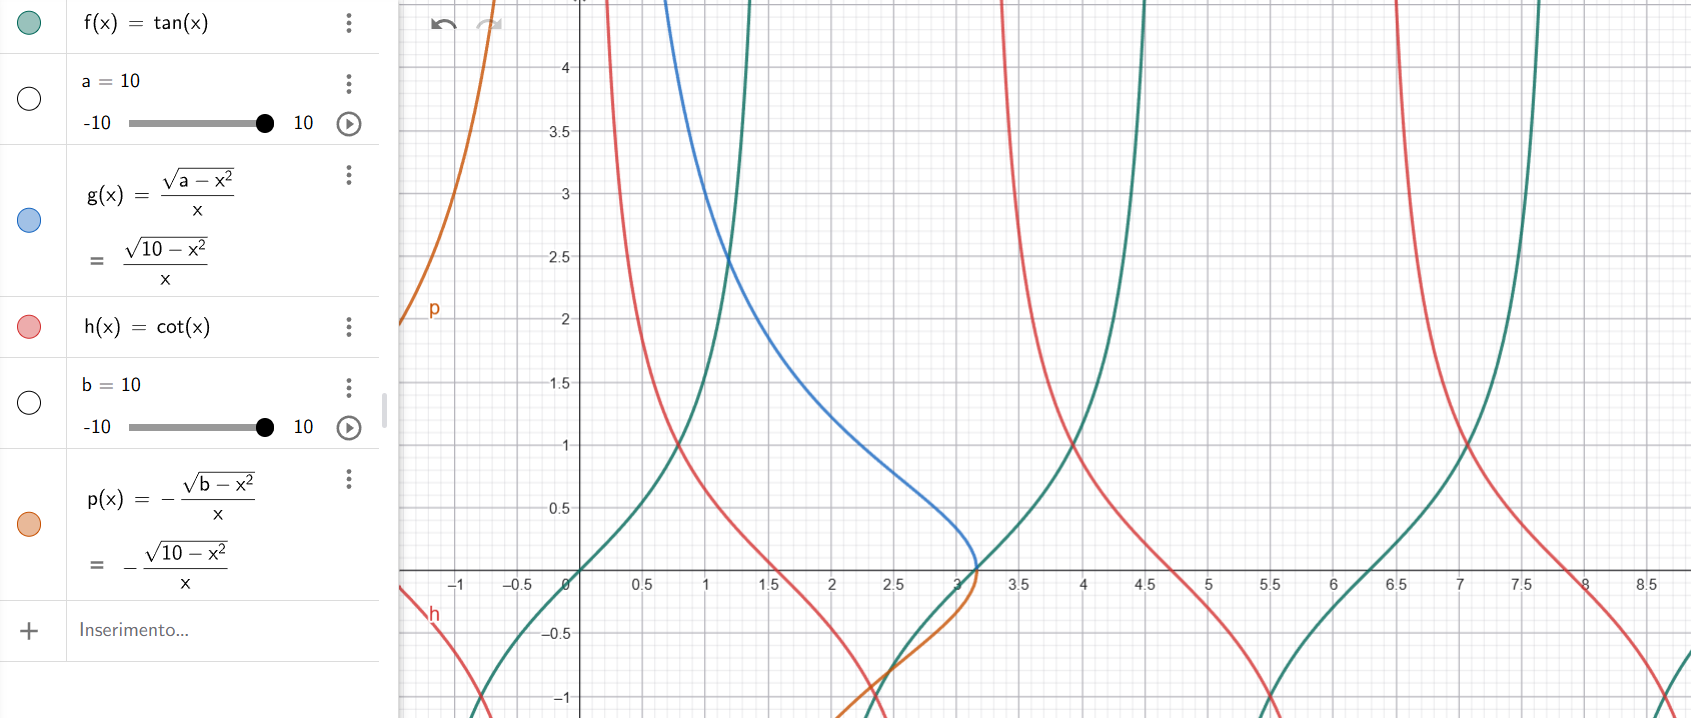
\includegraphics[width=0.9\linewidth]{immagini/Screenshot 2026-01-24 151007.png}
    \end{figure}
\end{center}
Dunque il numero di stati legati dipende dal parametro $\lambda$ e quindi dalla massa e dal potenziale. Tuttavia esiste sempre uno stato legato, indipendentemente da $\phi_0$ e $a$, infatti l'equazione trascendentale per le soluzioni pari ammette sempre almeno una soluzione.

\subsection{Potenziale delta}
Consideriamo il seguente potenziale
\begin{gather}
    \phi(x) = -\phi_0L\delta(x) \notag
\end{gather}
con $\phi_0, L > 0$. Fissiamo $E < 0$ e studiamo l'esistenza e la natura di eventuali stati legati. L'equazione alle autofunzioni è
\begin{gather}
    -\frac{\hbar^2}{2m}\frac{d^2}{dx^2}\psi(x) = (E + \phi_0L\delta(x))\psi(x) \notag
\end{gather}
anche in questo caso la derivata è discontinua, a causa del salto infinito del potenziale, infatti si ha
\begin{gather}
    -\frac{\hbar^2}{2m}\int_{-\varepsilon}^\varepsilon \frac{d^2}{dx^2}\psi(x) \, dx = -\frac{\hbar^2}{2m}(\psi'(\varepsilon) - \psi'(-\varepsilon)) = \int_{-\varepsilon}^\varepsilon(E + \phi_0L\delta(x))\psi(x) \, dx \notag
\end{gather}
ovvero per ogni $\varepsilon > 0$ si ha
\begin{gather}
    \psi'(\varepsilon) - \psi'(-\varepsilon) = -\frac{2m\phi_0L}{\hbar^2}\psi(0) \notag
\end{gather}
Per $x \neq 0$ si ha $\delta(x\neq0) = 0$, dunque otteniamo le seguenti soluzioni
\begin{gather}
    \begin{cases}
        \psi(x) = A_-e^{\beta x} \quad &x < 0 \\
        \psi(x) = A_+e^{-\beta x} \quad &x > 0
    \end{cases} \notag
\end{gather}
Imponendo la continuità in $x = 0$ si ottiene $A_- = A_+ (=: A)$, mentre imponendo che la discontinuità della derivata sia esattamente $\Delta \psi'(0) = -\frac{2m\phi_0L}{\hbar^2}$ si ottiene
\begin{gather}
    2\beta A = \frac{2m\phi_0L}{\hbar^2}A \notag
\end{gather}
ovvero esiste uno stato legato con energia
\begin{gather}
    |E| = \frac{\hbar^2 \beta^2}{2m} = \frac{m\phi_0^2L^2}{2\hbar^2} \notag
\end{gather}

\subsection{Barriera di potenziale}
Consideriamo il seguente potenziale
\begin{gather}
    \phi(x) = \begin{cases}
        \phi_0 \quad &x \in [0, L] \\
        0 \quad &x \not\in [0, L]
    \end{cases} \notag
\end{gather}
Siamo interessati a fenomeni di trasmissione e riflessione (di probabilità) in base ai parametri $\phi_0$ e $L$. Supponiamo sempre che l'onda incidente provenga da $-\infty$. \\ \\
Studiamo il caso $\phi_0, L > 0$. Fissiamo $0 < E < \phi_0$, la funzione d'onda della particella incidente prende la seguente forma
\begin{gather}
    \psi(x) = \begin{cases}
        Ae^{ikx} + Re^{-ikx} \quad &x < 0 \\
        c_+e^{\beta x} + c_e^{-\beta x} \quad &x \in [0, L] \\
        Te^{ikx} \quad &x > L 
    \end{cases} \notag
\end{gather}
A questo punto imponiamo la continuità per la funzione d'onda e la sua derivata
\begin{gather}
    \begin{cases}
        A + R = c_+ + c_- \\
        c_+e^{\beta L} + c_-e^{-\beta L} = Te^{ikL} \\
        ik\left( A - R \right) = \beta\left( c_+ - c_- \right) \\
        \beta\left( c_+e^{\beta L} -c_-e^{-\beta L} \right) = ikTe^{ikL}
    \end{cases} \implies 
    \begin{cases}
        A = \frac{1}{2}\left( 1 + \frac{\beta}{ik} \right)c_+ + \frac{1}{2}\left( 1 - \frac{\beta}{ik} \right)c_- \\
        R = \frac{1}{2}\left( 1 - \frac{\beta}{ik} \right)c_+ + \frac{1}{2}\left( 1 + \frac{\beta}{ik} \right)c_- \\
        c_+e^{\beta L} = \frac{1}{2}\left( 1 + \frac{ik}{\beta} \right)Te^{ikL} \\
        c_-e^{-\beta L} = \frac{1}{2}\left( 1 - \frac{ik}{\beta} \right)T^{ikL} 
    \end{cases} \notag
\end{gather}
dunque sostituendo si ottiene
\begin{gather}
    \begin{cases}
        A = \frac{1}{4}Te^{ikL}\left[ \left(1 + \frac{\beta}{ik} \right)\left( 1 + \frac{ik}{\beta} \right)e^{-\beta L} + \left( 1 - \frac{\beta}{ik} \right)\left( 1 - \frac{ik}{\beta} \right)e^{\beta L} \right] \\
        R = \frac{1}{4}Te^{ikL}\left[ \left( 1 - \frac{\beta}{ik} \right)\left( 1 + \frac{ik}{\beta} \right)e^{-\beta L} + \left( 1 + \frac{\beta}{ik} \right)\left( 1 - \frac{ik}{\beta} \right)e^{\beta L} \right]
    \end{cases} \notag
\end{gather}
ovvero
\begin{gather}
    \begin{cases}
        A = \frac{1}{4}Te^{ikL}\left[ \left( 2 + i\frac{k^2 - \beta^2}{k\beta} \right)e^{-\beta L} + \left( 2 - i\frac{k^2 - \beta^2}{k\beta} \right) e^{\beta L} \right] \\
        R = \frac{1}{4}iTe^{ikL}\left[ \left( \frac{\beta^2 + k^2}{k\beta} \right)e^{-\beta L} - \left( \frac{\beta^2 + k^2}{k\beta} \right)e^{\beta L} \right]
    \end{cases} \notag
\end{gather}
dunque
\begin{gather}
    \begin{cases}
        |A| = \frac{1}{4}T\left| 4\cos \beta L + 2\frac{k^2 - \beta^2}{k\beta}\sin \beta L \right| \\
        |R| = \frac{1}{4}T\left| 2\frac{\beta^2 + k^2}{k\beta}\sin \beta L \right|
    \end{cases} \notag
\end{gather}
quindi otteniamo le seguenti relazioni per i coefficienti delle onde
\begin{gather}
    \left| \frac{T}{A} \right| = \frac{1}{\left| \cos \beta L + \frac{k^2 - \beta^2}{2k\beta}\sin \beta L \right|} \qquad \left| \frac{R}{A} \right| = \left| \frac{\frac{\beta^2 + k^2}{k\beta}\sin \beta L}{2\cos \beta L + \frac{k^2 - \beta^2}{k\beta}\sin \beta L} \right| \notag
\end{gather}
Fissiamo ora $0 < \phi_0 < E$, la funzione d'onda della particella incidente prende la seguente forma
\begin{gather}
    \phi(x) = \begin{cases}
        Ae^{ikx} + Re^{-ikx} \quad &x < 0 \\
        Ce^{i\tilde{k}x} + \tilde{R}e^{-i\tilde{k}x} \quad &x \in [0, L] \\
        Te^{ikx} \quad &x > L
    \end{cases} \notag
\end{gather}
dove $k > \tilde{k}$, infatti
\begin{gather}
    k = \frac{\sqrt{2mE}}{\hbar} \quad \tilde{k} = \frac{\sqrt{2m(E - \phi_0)}}{\hbar} \notag
\end{gather}
Imponiamo la continuità della funzione d'onda e della sua derivata
\begin{gather}
    \begin{cases}
        A + R = C + \tilde{R} \\
        Ce^{i\tilde{k}L} + \tilde{R}e^{-i\tilde{k}L} = Te^{ikL} \\
        ik\left( A - R \right) = i\tilde{k}( C - \tilde{R} ) \\
        i\tilde{k}(Ce^{i\tilde{k}L} - \tilde{R}e^{-i\tilde{k}L}) = ikTe^{ikL}
    \end{cases} \implies
    \begin{cases}
        A = \frac{1}{2}\left( 1 + \frac{\tilde{k}}{k} \right)C + \frac{1}{2}\left( 1 - \frac{\tilde{k}}{k} \right)\tilde{R} \\
        R = \frac{1}{2}\left( 1 - \frac{\tilde{k}}{k} \right)C + \frac{1}{2}\left( 1 + \frac{\tilde{k}}{k} \right)\tilde{R} \\
        Ce^{i\tilde{k}L} = \frac{1}{2}\left( 1 + \frac{k}{\tilde{k}} \right)Te^{ikL} \\
        \tilde{R}e^{-i\tilde{k}L} = \frac{1}{2}\left( 1 - \frac{k}{\tilde{k}} \right)Te^{ikL}
    \end{cases} \notag
\end{gather}
dunque sostituendo si ottiene
\begin{gather}
    \begin{cases}
        A = \frac{1}{4}Te^{ikL}\left[ \left( 1 + \frac{\tilde{k}}{k} \right)\left( 1 + \frac{k}{\tilde{k}} \right)e^{-i\tilde{k}L} + \left( 1 - \frac{\tilde{k}}{k} \right)\left( 1 - \frac{k}{\tilde{k}} \right)e^{i\tilde{k}L} \right] \\
        R = \frac{1}{4}Te^{ikL}\left[ \left( 1 - \frac{\tilde{k}}{k} \right)\left( 1 + \frac{k}{\tilde{k}} \right)e^{-i\tilde{k}L} + \left( 1 + \frac{\tilde{k}}{k} \right)\left( 1 - \frac{k}{\tilde{k}} \right)e^{i\tilde{k}L} \right] 
    \end{cases} \notag
\end{gather}
ovvero
\begin{gather}
    \begin{cases}
        A = \frac{1}{4}Te^{ikL}\left[ \left( 2 + \frac{k^2 + \tilde{k}^2}{k\tilde{k}} \right)e^{-i\tilde{k}L} + \left( 2 - \frac{k^2 + \tilde{k}^2}{k\tilde{k}} \right)e^{i\tilde{k}L} \right] \\
        R = \frac{1}{4}Te^{ikL}\left[ \left( \frac{k^2 - \tilde{k}^2}{k\tilde{k}} \right)e^{-i\tilde{k}L} - \left( \frac{k^2 - \tilde{k}^2}{k\tilde{k}} \right)e^{i\tilde{k}L} \right]
    \end{cases} \notag
\end{gather}
dunque
\begin{gather}
    \begin{cases}
        |A| = \frac{1}{4}T\left| 4\cos \tilde{k}L - 2i\frac{k^2 + \tilde{k}^2}{k\tilde{k}}\sin \tilde{k} L \right| \\
        |R| = \frac{1}{4}T\left| 2\frac{k^2 - \tilde{k}^2}{k\tilde{k}}\sin \tilde{k}L \right|
    \end{cases} \notag
\end{gather}
quindi otteniamo le seguenti relazioni per i coefficienti delle onde
\begin{gather}
    \left| \frac{T}{A} \right| = \frac{1}{\left| \cos \tilde{k}L - i\frac{k^2 + \tilde{k}^2}{k\tilde{k}}\sin \tilde{k}L \right|} \qquad
    \left| \frac{R}{A} \right| = \left| \frac{\frac{k^2 - \tilde{k}^2}{2k\tilde{k}}\sin \tilde{k}L}{\cos \tilde{k}L - i\frac{k^2 + \tilde{k}^2}{2k\tilde{k}}\sin \tilde{k}L} \right| \notag
\end{gather} 

\subsection{Potenziale lineare}
Consideriamo il seguente potenziale
\begin{gather}
    \phi(x) = k|x| \notag
\end{gather}
esso ammette stati legati per ogni energia $E$ fissata, dunque ci aspettiamo normalizzazione. L'equazione alle autofunzioni diventa
\begin{gather}
    -\frac{\hbar^2}{2m}\frac{d^2}{dx^2}\psi(x) + k|x|\psi(x) = E\psi(x) \notag
\end{gather}
per rimuovere il problema del valore assoluto osserviamo che il potenziale è una funzione pari, possiamo dunque considerare solamente $x \geq 0$, per la simmetria avremo soluzioni pari e soluzioni dispari. Definendo $s = x - \frac{E}{k}$ si ottiene
\begin{gather}
    -\frac{\hbar^2}{2m}\frac{d^2}{ds^2}\psi(s) + ks\psi(s) = 0 \notag
\end{gather}
nella base degli impulsi l'equazione diventa
\begin{gather}
    \frac{1}{2m}p^2\psi(p) + i\hbar k\frac{d}{dp}\psi(p) = 0 \notag
\end{gather}
che ha come soluzione
\begin{gather}
    \psi(p) = \psi(0)e^{\frac{ip^3}{6m\hbar k}} \notag
\end{gather}
passando in base $s$ tramite antitrasformata di Fourier si ottiene
\begin{gather}
    \psi(s) = \int_{\mathbf{R}}dp\, \frac{1}{\sqrt{2\pi\hbar}}e^{\frac{ips}{\hbar}}e^{\frac{ip^3}{6m\hbar k}} \notag
\end{gather}
possiamo supporre che le autofunzioni siano reali, pertanto si ottiene
\begin{gather}
    \psi(s) = \int_{\mathbf{R}}dp \, \frac{1}{\sqrt{2\pi\hbar}}\cos\left( \frac{p^3}{6m\hbar k} + \frac{ps}{\hbar} \right) \notag
\end{gather}
ovvero l'autofunzione in base $x$ è la funzioni di Airy, oscillante prima del punto di inversione del moto ed esponenzialmente soppressa dopo (ricordiamo che nella variabile $s$ il punto di inversione del moto ad $E$ fissato è l'origine).

\subsection{Approssimazione WKB}
Consideriamo la funzione d'onda $\braket{x|\psi}$ associata ad un stato stazionario $\ket{\psi}$. In generale $\braket{x|\psi} \in \mathbf{C}$, dunque può essere espressa in forma polare
\begin{gather}
    \psi(x) = Ae^{i\phi} \tag{7.6.1}
\end{gather}
dove $A$ e $\phi$ sono funzioni reali di $x$, pertanto si ha
\begin{align}
    \psi' &= (A' + i\phi')e^{i\phi} \tag{7.6.2.a} \\
    \psi'' &= (A'' + 2iA'\phi' + i\phi''A - \phi'^2A)e^{i\phi} \tag{7.6.2.b}
\end{align}
Definiamo $p(x) = \sqrt{2m(E - V(x))}$, l'equazione di Schrodinger indipendente dal tempo è data da
\begin{gather}
    \psi'' = -\frac{p^2}{\hbar^2}\psi \tag{7.6.3}
\end{gather}
pertanto sostituendo $(7.6.1)$ e $(7.6.2.b)$ in $(7.6.3)$ si ottiene
\begin{gather}
    A'' + 2iA'\phi' + i\phi''A - \phi'^2A = -\frac{p^2}{\hbar^2}A \notag
\end{gather}
Separando parte reale e immaginaria dell'equazione si ottengono due equazioni differenziali reali
\begin{align}
    Re:& \qquad A'' - \phi'^2A = -\frac{p^2}{\hbar^2}A \notag \\
    Im:& \qquad \phi''A + 2A'\phi' = 0 \notag
\end{align}
che sono equivalenti a
\begin{align}
    Re:& \qquad A'' = A\left( \phi'^2 - \frac{p^2}{\hbar^2} \right) \tag{7.6.4.a} \\
    Im:& \qquad \left( A^2\phi' \right)' = 0 \tag{7.6.4.b}
\end{align}
equazione $(7.6.4.b)$ si risolve immediatamente
\begin{gather}
    A^2\phi' = c \implies A = \frac{c}{\sqrt{\phi'}} \notag
\end{gather}
equazione $(7.6.4.a)$ non può essere risolta esattamente, supponiamo allora che $A$ vari abbastanza lentamente da poter trascurare $A''/A$ rispetto agli altri termini, allora si ha
\begin{gather}
    (\phi')^2 = \frac{p^2}{\hbar^2} \implies \phi = \pm\frac{1}{\hbar}\int dx \, p(x) \notag
\end{gather}
questo ci permette di determinare la forma approssimata dell'autofunzione $\psi(x)$, data da
\begin{gather}
    \psi(x) \sim \pm\frac{c}{\sqrt{p(x)}}e^{\pm\frac{i}{\hbar}\int dx \, p(x)} \notag
\end{gather}
notiamo che
\begin{gather}
    |\psi(x)|^2 \sim \frac{c^2}{p(x)} \notag
\end{gather}
ovvero l'ampiezza di probabilità di trovare la particella è inversamente proporzionale al suo impulso classico. \\ \\
\textbf{Esempio: buca di potenziale (non costante) infinita:} consideriamo il seguente potenziale
\begin{gather}
    \phi(x) = \begin{cases}
        f(x) \quad &0 < x < a \\
        \infty \quad &\text{altrimenti}
    \end{cases} \notag 
\end{gather}
dove $a > 0$ e $f$ è una qualsiasi funzione continua. Per $x \in (0, a)$ si ha
\begin{gather}
    \psi(x) \sim \frac{1}{\sqrt{p(x)}}\left( c_+e^{i\phi(x)} + c_-e^{-i\phi(x)} \right) \notag 
\end{gather}
dove
\begin{gather}
    \phi(x) = \int_0^x dx' \, p(x') \notag
\end{gather}
Ora $\psi(x)$ deve essere nulla per $x = 0$ e, poiché $\phi(0) = 0$, si ha $c_+ = - c_-$, ovvero
\begin{gather}
    \psi(x) \sim \frac{2i}{\sqrt{p(x)}}c_+\sin\phi(x) \notag
\end{gather}
Inoltre, $\psi(a) = 0$, pertanto $\phi(a) = n\pi$, concludiamo che
\begin{gather}
    \int_0^a dx \, p(x) = n\pi\hbar \notag
\end{gather}
questa è la condizione di quantizzazione che determina i livelli energetici approssimati. \\ \\
Tuttavia, a meno che non consideriamo potenziale infinito al di fuori di una regione limitata dello spazio e dunque imponiamo che la funzione d'onda sia ivi nulla, l'approssimazione WKB fallisce vicino ai punti di inversione del moto, dove $p(x) = 0$. Dobbiamo allora trovare una correzione all'approssimazione per connettere la soluzione della regione classicamente permessa con la soluzione della regione classicamente proibita. \\
Trasliamo lo spazio in modo tale che il punto di inversione del moto occorra a $x = 0$, si ha che
\begin{gather}
    \psi(x) \sim \begin{cases}
        \frac{1}{\sqrt{p(x)}}\left( A_1e^{\frac{i}{\hbar}\int_x^0 dx' \, p(x')} + B_1e^{-\frac{i}{\hbar}\int_x^0 dx' \, p(x')} \right) \quad &x < 0 \\
        \frac{1}{\sqrt{|p(x)|}}A_2e^{-\frac{1}{\hbar}\int_0^x dx' \, |p(x')|} \quad &x > 0 
    \end{cases} \notag
\end{gather}
assumento che $V(x) > E$ per ogni $x > 0$. Poiché la correzione è necessaria solamente per un intorno abbastanza piccolo del punto di inversione del moto, possiamo introdurre una funzione d'onda correttiva $\psi_p$, che connette le funzioni d'onda delle due regioni. Tale funzione è definita in un intorno dove è possibile approssimare il potenziale con una retta
\begin{gather}
    V(x) \sim E + V'(0)x \notag
\end{gather}
l'equazione di Schrodinger per il potenziale linearizzato diventa
\begin{gather}
    -\frac{\hbar^2}{2m}\frac{d^2\psi_p}{dx^2} + (E + V'(0)x)\psi_p = E\psi_p \notag
\end{gather}
definendo $\alpha = \left( \frac{2m}{\hbar^2}V'(0) \right)^{1/3}$ si ha
\begin{gather}
    \frac{d^2\psi_p}{dx^2} = \alpha^3x\psi_p \notag
\end{gather}
pertanto la variabile $x$ può essere sostituita dalla variabile indipendente $z = \alpha x$. L'equazione in termini di $z$ diventa
\begin{gather}
    \frac{d^2\psi_p}{dz^2} = z\psi_p \notag
\end{gather}
ovvero l'equazione di Airy, che ha come soluzioni le funzioni di Airy. A questo punto dobbiamo connettere le funzioni d'onda nelle due regioni con $\psi_p$ in modo tale che la funzione d'onda risultante sia continua. Nelle regioni di connessione vale ancora l'approssimazione lineare del potenziale, dunque
\begin{gather}
    p(x) \sim \sqrt{2m(E - E - V'(0)x} = \hbar\alpha^{2/3}\sqrt{-x} \notag
\end{gather}
nella regione di connessione tra $\psi_p$ e la soluzione $WKB$ esponenzialmente soppressa $(x > 0)$ si ha
\begin{gather}
    \int_0^x dx \, |p(x')| \sim \hbar\alpha^{2/3}\int_0^x dx \, \sqrt{x'} = \frac{2}{3}\hbar(\alpha x)^{2/3} \notag
\end{gather}
dunque la soluzione WKB in tale regione di connessione prende la seguente forma
\begin{gather}
    \psi(x) \sim \frac{D}{\sqrt{\hbar}\alpha^{3/4}x^{1/4}}e^{-\frac{2}{3}(\alpha x)^{3/2}} \tag{7.6.5}
\end{gather}
confrontando con la forma asintotica per $z >> 0$ della funzione di Airy, data da
\begin{align}
    Ai(z) &\sim \frac{1}{2\sqrt{\pi}z^{1/4}}e^{-\frac{2}{3}z^{3/2}} \notag \\
    Bi(z) &\sim \frac{1}{\sqrt{\pi}z^{1/4}}e^{\frac{2}{3}z^{3/2}} \notag
\end{align}
otteniamo che la funzione di connessione è della forma
\begin{gather}
    \psi_p(x) \sim \frac{a}{2\sqrt{\pi}(\alpha x)^{1/4}}e^{-\frac{2}{3}(\alpha x)^{3/2}} + \frac{b}{\sqrt{\pi}(\alpha x)^{1/4}}e^{\frac{2}{3}(\alpha x)^{3/2}} \notag
\end{gather}
confrontando con $(7.6.5)$ si ha che
\begin{gather}
    a = \sqrt{\frac{4\pi}{\alpha\hbar}}D \quad b = 0 \tag{7.6.6}
\end{gather}
Ora ripetiamo il procedimento per la regione di connessione tra la soluzione WKB oscillante e la funzione di Airy $(x < 0)$, si ha che
\begin{gather}
    \int_0^x dx' \, p(x') \sim \frac{2}{3}\hbar(-\alpha x)^{3/2} \notag
\end{gather}
dunque la funzione WKB prende la seguente forma
\begin{gather}
    \psi(x) \sim \frac{1}{\sqrt{\hbar}\alpha^{3/4}(-x)^{1/4}}\left( Be^{i\frac{2}{3}(-\alpha x)^{3/2}} + Ce^{-i\frac{2}{3}(-\alpha x)^{3/2}} \right) \tag{7.6.7}
\end{gather}
Mentre usando la forma asintontica della funzione di Airy per $z << 0$, data da
\begin{align}
    Ai(z) &\sim \frac{1}{\sqrt{\pi}(-z)^{1/4}}\sin\left( \frac{2}{3}(-z)^{3/2} + \frac{\pi}{4} \right) \notag \\
    Bi(z) &\sim \frac{1}{\sqrt{\pi}(-z)^{1/4}}\cos\left( \frac{2}{3}(-z)^{3/2} + \frac{\pi}{4} \right) \notag
\end{align}
otteniamo che la funzione di connessione è della forma
\begin{gather}
    \psi_p(x) \sim \frac{a}{\sqrt{\pi}(-z)^{1/4}}\sin\left( \frac{2}{3}(-z)^{3/2} + \frac{\pi}{4} \right) \notag
\end{gather}
dove abbiamo sempre posto $b = 0$, pertanto confrontando con $(7.6.7)$ otteniamo
\begin{gather}
    B = -ie^{i\frac{\pi}{4}}D \quad C = ie^{i\frac{\pi}{4}}D \notag
\end{gather}
dove è stata sostituita l'espressione di $a$ in $(7.6.6)$. Ha senso usare la forma asintotica della funzione di Airy poiché la variabile in questo caso è $\alpha x$, con $\alpha$ termine molto grande in modulo. Traslando nuovamente lo spazio in modo tale che il punto di inversione del moto sia un generico punto $x_2$, la soluzione WKB diventa
\begin{gather}
    \psi(x) \sim \begin{cases}
        \frac{2D}{\sqrt{p(x)}}\cos\left( \frac{1}{\hbar}\int_x^{x_2} dx' \, p(x') - \frac{\pi}{4} \right) \quad &x < x_2 \\
        \frac{D}{\sqrt{|p(x)|}}\exp\left( -\frac{1}{\hbar}\int_{x_2}^x dx' \, |p(x')| \right) \quad &x > x_2
    \end{cases} \notag
\end{gather}
Questo è il caso in cui il potenziale cresce in un intorno del punto di inversione del moto. Lo stesso ragionamento applicato al caso in cui il potenziale decresce in un intorno del punto di inversione del moto fornisce
\begin{gather}
    \psi(x) \sim \begin{cases}
        \frac{D'}{\sqrt{|p(x)|}}\exp\left( -\frac{1}{\hbar}\int_x^{x_1} dx' \, |p(x')| \right) \quad &x < x_1 \\
        \frac{2D'}{\sqrt{p(x)}}\cos\left( \frac{1}{\hbar}\int_{x_1}^x dx' \, p(x') - \frac{\pi}{4} \right) \quad &x > x_1
    \end{cases} \notag
\end{gather}
Gli argomenti del coseno devono essere uguali e quindi differire al più di un termine $n\pi$ (non $2n\pi$ poiché un segno meno può sempre essere inglobato nella costante di normalizzazione), ovvero deve valere
\begin{gather}
    \frac{1}{\hbar}\int_x^{x_2}dx' \, p(x') + \frac{1}{\hbar}\int_{x_1}^x dx' \, p(x') = n\pi + \frac{\pi}{2} \notag
\end{gather}
che ci porta alla condizione di quantizzazione di Bohr - Sommerfeld 
\begin{gather}
    \int_{x_1}^{x_2}dx \, p(x) = \pi\hbar\left( n + \frac{1}{2} \right) \notag
\end{gather}

\newpage
\section{Teoria delle perturbazioni}
Tratteremo ora metodi di approssimazione per problemi che non possono essere risolti esattamente, che però possono essere trattati come problemi risolubili a cui viene aggiunta una perturbazione.

\subsection{Teoria delle perturbazioni indipendenti dal tempo: caso non degenere}
Consideriamo un hamiltoniano indipendente dal tempo $H$ che possa essere separato in due termini
\begin{gather}
    H = H_0 + V \notag
\end{gather}
dove $H_0$ è detto hamiltoniano imperturbato e $V$ è detta perturbazione, e supponiamo che il problema $V = 0$ si possa risolvere esattamente, ovvero che si conoscano gli autovalori $E_n^0$ e gli autostati $\ket{n^0}$ dell'hamiltoniano imperturbato
\begin{gather}
    H_0\ket{n^0} = E_n^0\ket{n^0} \notag
\end{gather}
l'insieme degli autostati di $H_0$ è completo e vale la relazione $\sum_n \ket{n^0}\bra{n^0} = 1$. Inoltre supponiamo che lo spettro di energia sia discreto. Introduciamo il parametro continuo $\lambda \in [0, 1]$ e consideriamo l'hamiltoniano
\begin{gather}
    H = H_0 + \lambda V \notag
\end{gather}
dove $H = H_\lambda$. L'idea è quella di sviluppare gli autovalori $E_n$ e gli autostati $\ket{n}$ dell'hamiltoniano $H$ in potenze di $\lambda$. In particolare ci aspettiamo che
\begin{align}
    \lim_{\lambda \rightarrow 0} \ket{n} &= \ket{n^0} \notag \\
    \lim_{\lambda \rightarrow 0} \Delta_n &= 0 \notag
\end{align}
dove $\Delta_n = E_n - E_n^0$, variazione in energia del livello $n$-esimo a causa della perturbazione $V$. L'equazione di Schrodinger indipendente dal tempo è
\begin{gather}
    (H_0 + \lambda V)\ket{n} = E_n\ket{n} \notag
\end{gather}
che può essere riscritta come
\begin{gather}
    (E_n^0 - H_0)\ket{n} = (\lambda V - \Delta_n)\ket{n} \tag{8.1.1}
\end{gather}
Potrebbe sembrare ragionevole invertire l'operatore $E_n^0 - H_0$, tuttavia ovviamente $E_n^0 \in \sigma(H_0)$ pertanto non è ben definito l'inverso. Fortunatamente si ha
\begin{gather}
    \braket{n^0|\lambda V - \Delta_n|n} = 0 \tag{8.1.2}
\end{gather}
infatti moltiplicando $(8.1.1)$ a sinistra per $\bra{n^0}$ si ha
\begin{gather}
    \braket{n^0|E_n^0 - H_0|n} = E_n^0\braket{n^0|n} - E_n^0\braket{n^0|n} = 0 \notag
\end{gather}
definendo l'operatore di proiezione complementare
\begin{gather}
    \phi_n = 1 - \ket{n^0}\bra{n^0} = \sum_{k \neq n} \ket{k^0}\bra{k^0} \notag
\end{gather}
si ha che l'operatore
\begin{gather}
    (E_n^0 - H_0)^{-1}\phi_n = \sum_{k \neq n} \frac{1}{E_n^0 - E_k^0} \ket{k^0}\bra{k^0} \notag
\end{gather}
è ben definito, poiché $\phi_n$ manda tutto lo spazio di Hilbert nel sottospazio ortogonale a $\ket{n^0}$. Segue che
\begin{gather}
    (\lambda V - \Delta_n)\ket{n} = \phi_n(\lambda V - \Delta_n)\ket{n} \notag
\end{gather}
banalmente. Viene naturale allora pensare che
\begin{gather}
    \ket{n} = c_n(\lambda)\ket{n^0} + (E_n^0 - H_0)^{-1}\phi_n(\lambda V - \Delta_n)\ket{n} \tag{8.1.3}
\end{gather}
dove
\begin{gather}
    \lim_{\lambda \rightarrow 0} c_n(\lambda) = 1 \notag
\end{gather}
in questo modo $\ket{n} \rightarrow \ket{n^0}$ per $\lambda \rightarrow 0$. Notiamo che
\begin{gather}
    c_n(\lambda) = \braket{n^0|n} \notag
\end{gather}
In realtà è conveniente supporre che $c_n = 1$ anche per $\lambda \neq 0$, abbandonando la convenzione di normalizzazione degli stati. Infatti porre $c_n \neq 1$ ha come unico effetto un fattore moltiplicativo costante, tuttavia è sempre possibile normalizzare gli stati a conti fatti. \\ \\
Da $(8.1.2)$ si ha che
\begin{gather}
    \Delta_n = \lambda\braket{n^0|V|n} \tag{8.1.4}
\end{gather}
A questo punto sviluppiamo in potenze di $\lambda$ autovalori e autostati
\begin{align}
    \Delta_n &= \lambda\Delta_n^1 + \lambda^2\Delta_n^2 + \dots \notag \\
    \ket{n} &= \ket{n^0} + \lambda\ket{n^1} + \lambda^2\ket{n^2} + \dots \notag
\end{align}
sostituendo in $(8.1.4)$ e confrontando i termini con potenze uguali di $\lambda$ otteniamo le correzioni ai livelli energici
\begin{align}
    O(\lambda):& \qquad \Delta_n^1 = \braket{n^0|V|n^0} \notag \\
    O(\lambda^2):& \qquad \Delta_n^2 = \braket{n^0|V|n^1} \notag \\
    . \notag \\
    . \notag \\
    O(\lambda^N):& \qquad \Delta_n^N = \braket{n^0|V|n^N} \notag
\end{align}
pertanto è sufficiente conoscere la correzione di ordine $k - 1$ degli autostati per conoscere la correzione di ordine $k$ degli autovalori. A questo punto sostituendo in $(8.1.3)$ otteniamo le correzioni agli autostati
\begin{align}
    O(\lambda):& \qquad \ket{n^1} = (E_n^0 - H_0)^{-1}\phi_nV\ket{n^0} \notag \\
    O(\lambda^2):& \qquad \ket{n^2} = \frac{\phi_n}{E_n^0 - H_0}V\ket{n^1} - \frac{\phi_n}{E_n^0 - H_0}\Delta_n^1\ket{n^1} \notag
\end{align}
dove si è usato $\phi_n\ket{n^0} = 0$. 

\subsection{Teoria delle perturbazioni indipendenti dal tempo: caso degenere}
Nel caso in cui l'hamiltoniano imperturbato $H_0$ ha autovalori degeneri la trattazione precedente non è più valida, infatti non è più chiaro a che combinazione lineare di autostati dello spazio degenere converga l'autostato perturbato per $\lambda \rightarrow 0$. \\ \\
Distinguiamo con un secondo indice gli autostati del sottospazio degenere $D$, si ha
\begin{align}
    H_0\ket{n^0; \tilde{i}} &= E_D^0\ket{n^0; \tilde{i}} \notag \\
    \braket{n^0; \tilde{j}|n^0; \tilde{i}} &= \delta_{\tilde{i}\tilde{j}} \notag
\end{align}
con $1 \leq i \leq s_n$, dove $s_n$ indica il grado di degenerazione dell'$n$-esimo livello energetico. La tilde sull'indice sta a significare che la scelta degli autostati nel sottospazio degenere è del tutto arbitraria, infatti qualsiasi combinazione lineare è autostato con autovalore $E_D^0$ (tutto il sottospazio degenere è formato da autostati con autovalore $E_D^0$). \\ \\
Tuttavia la scelta degli autostati perturbati $\ket{n}$ non è arbitraria, infatti deve sempre valere
\begin{gather}
    \lim_{\lambda \rightarrow 0}\ket{n} = \ket{n^0} \notag
\end{gather}
ora sviluppiamo $\ket{n}$ in potenze di $\lambda$ nel sottospazio degenere
\begin{align}
    \ket{n} &= \ket{n^0} + \lambda\ket{n^1} + \dots \notag \\
    &= \sum_{i = 1}^{s_n}\alpha_{n, i}\ket{n^0; \tilde{i}} + \lambda\sum_{k \neq n}c_{nk}^{(1)}\sum_{i = 1}^{s_n}\alpha_{k, i}\ket{k^0; \tilde{i}} + \dots \notag
\end{align}
dove abbiamo supposto che $\braket{n^0, n^1} = 0$, che è ragionevole in quanto una correzione sulla stessa direzione di $\ket{n^0}$ non aggiungerebbe nessuna informazione allo stato. \\
Considerando per semplicità solamente la correzione al primo ordine in $\lambda$ e sostituendo nell'equazione di Schrodinger indipendente dal tempo si ottiene
\begin{align}
    (H_0 + \lambda V)&\left( \sum_{i = 1}^{s_n}\alpha_{n, i}\ket{n^0; \tilde{i}} + \lambda\sum_{k \neq n}c_{nk}^{(1)}\sum_{i = 1}^{s_n}\alpha_{k, i}\ket{k^0; \tilde{i}} \right) \notag \\
    &= (E_D^0 + \lambda E_D^1)\left( \sum_{i = 1}^{s_n}\alpha_{n, i}\ket{n^0; \tilde{i}} + \lambda\sum_{k \neq n}c_{nk}^{(1)}\sum_{i = 1}^{s_n}\alpha_{k, i}\ket{k^0; \tilde{i}} \right) \notag
\end{align}
facendo il prodotto scalare con $\ket{n^0; \tilde{j}}$ si ha
\begin{gather}
    \sum_{i = 1}^{s_n}\braket{n^0; \tilde{j}|V|n^0; \tilde{i}}\alpha_{n, i} = E_D^1\alpha_{n, j} \tag{8.2.1}
\end{gather}
in particolare la $(8.2.1)$ è soddisfatta se $V$ è diagonale nella base provvisoria e se $E_D^1$ è un autovalore. Pertanto le soluzioni sono date dall'equazione secolare, che ha $s_n$ soluzioni, in genere differenti, che sono le correzioni al primo ordine dell'energia
\begin{gather}
    \det(V_{ji} - E_D^1\delta_{ji}) = 0 \notag
\end{gather}
Noti gli autovalori possiamo determinare la corretta base dello spazio degenere da utilizzare. Se le soluzioni al primo ordine non sono distinte è necessario diagonalizzare la matrice al secondo ordine.

\subsection{Applicazioni}
Vediamo qualche applicazione della teoria delle perturbazioni indipendente dal tempo.

\subsubsection{Effetto Stark}
Consideriamo l'hamiltoniano di un atomo idrogenoide soggetto ad un campo elettrico $\vec{\mathcal{E}}$ costante, diretto nella direzione positiva $\hat{z}$
\begin{gather}
    H = H_0 + H_S \notag
\end{gather}
dove $H_S = -\vec{\mu}_{el} \cdot \vec{\mathcal{E}} = e\mathcal{E}z = e\mathcal{E}r\cos\theta$. La perturbazione $H_S$ è un operatore dispari sotto trasformazioni di parità, infatti
\begin{gather}
    \cos(\pi - \theta) = -\cos\theta \notag
\end{gather}
si ha che gli elementi diagonali della matrice di perturbazione sono nulli. Ad esempio
\begin{align}
    \braket{100|H_S|100} &= e\mathcal{E}\braket{100|r\cos\theta|100} \notag \\
    &= \int_0^\infty dr \, r^2|R_{10}(r)|^2r \int_0^\pi d\theta \, \sin\theta\cos\theta \int_0^{2\pi} d\varphi \, |Y^0_0|^2 \notag = 0
\end{align}
perché ponendo $s = \sin\theta$, dunque $ds = \cos\theta d\theta$, si ha
\begin{gather}
    \int_0^\pi d\theta \, \sin\theta\cos\theta = \int_0^0 dx \, x = 0 \notag
\end{gather}
Pertanto per energie non degeneri la prima correzione non nulla è al secondo ordine in $\lambda$, per il quale si ha
\begin{align}
    E_{100}^{(2)} = e^2\mathcal{E}^2\sum_{k \neq 100} \frac{|\braket{k^0|z|100}|^2}{E_{100}^{(0)} - E_k^{(0)}} \notag
\end{align}
poiché $z = r\cos\theta$ è proporzionale a $Y^1_0$ si ha che contribuiscono solamente autostati $\ket{n10}$ con $n \geq 2$ alla somma. \\ \\
Nel sottospazio degenere determiniamo gli autovalore e gli autovettori della matrice perturbativa. Notiamo che $[H_S, L_z] = 0$, dunque
\begin{align}
    0 = \braket{nl'm'|[z, L_z]|nlm} &= \braket{nl'm'|zL_z - L_zz|nlm} \notag \\
    &= \hbar(m' - m)\braket{nl'm'|z|nlm} \notag
\end{align}
dunque sono nulli gli elementi di matrice $m \neq m'$ e $l = l'$.

\subsubsection{Correzione relativistica dell'energia cinetica}
L'energia relativistica di una particella è data da
\begin{align}
    E &= \sqrt{m^2c^4 + p^2c^2} \notag \\
    &= mc^2\sqrt{\left( 1 + \frac{p^2}{m^2c^2} \right)} \notag \\
    &\sim mc^2\left( 1 + \frac{p^2}{2m^2c^2} - \frac{p^4}{8m^4c^4} + \dots \right) \notag \\
    &\sim mc^2 + \frac{p^2}{2m} - \frac{p^4}{8m^3c^4} \notag
\end{align}
il primo termine è l'energia a riposo della particella ($m$ massa a riposo), dunque trasla semplicemente lo zero dell'energia ma non influisce su variazioni di energia. Il secondo termine è l'energia cinetica classica della particella. Il terzo termine è la prima correzione relativistica. \\
L'effetto della correzione relativistica sui livelli energetici atomici può essere trattato come una perturbazione indipendente dal tempo dell'hamiltoniano, poniamo allora $H_{cin} = -\frac{p^4}{8m^3c^2}$, notiamo che
\begin{align}
    H_{cin} &= -\frac{p^4}{8m^3c^2} \notag \\
    &= -\frac{1}{2mc^2}\left( \frac{p^2}{2m} \right)^2 \notag \\
    &= -\frac{1}{2mc^2}\left( H_0 + \frac{Ze^2}{r} \right)^2 \notag \\
    &= -\frac{1}{2mc^2}\left( H_0^2 + \frac{Z^2e^4}{r^2} + H_0\frac{Ze^2}{r} + \frac{Ze^2}{r}H_0 \right) \notag
\end{align}
La perturbazione $H_{cin}$ è diagonale in base $\ket{nlm}$ dunque si ha
\begin{align}
    E_{cin}^{(1)} &= \braket{nlm|H_{cin}|nlm} \notag \\
    &= -\frac{1}{2mc^2}\left( E_n^2 + Z^2e^4\braket{\frac{1}{r^2}}_{nl} + 2E_nZ^2e^4\braket{\frac{1}{r}}_{nl} \right) \notag
\end{align}


\subsection{Teoria delle perturbazione dipendenti dal tempo}
Consideriamo ora il caso in cui la perturbazione $V$ dipende esplicitamente dal tempo $V = V(t)$, dunque
\begin{gather}
    H = H_0 + \lambda V(t) \notag
\end{gather}
e vogliamo risolvere
\begin{gather}
    \begin{cases}
        i\hbar\frac{\partial \psi}{\partial t} = (H_0 + \lambda V)\psi \\
        \psi(x, 0) = \phi(x) 
    \end{cases} \notag
\end{gather}
per qualsiasi istante $t$ le autofunzioni di $H_0$ formano una base ortonormale, pertanto possiamo scrivere
\begin{gather}
    \psi(x, t) = \sum_{n} c_n(t)e^{-i\frac{E^0_n}{\hbar}t}\psi_n(x) \notag
\end{gather}
sostituendo nell'equazione di Schrodinger si ottiene
\begin{gather}
    \begin{cases}
        \sum_n\left( i\hbar\frac{\partial c_n}{\partial t} + \cancel{E^0_nc_n(t)}\right)e^{-i\frac{E^0_n}{\hbar}t}\psi_n(x) = (\cancel{H_0} + \lambda V)\sum_n c_n(t)e^{-i\frac{E^0_n}{\hbar}t}\psi_n(x) \\
        \psi(x, 0) = \phi(x) = \sum_n c_n(0)\psi_n(x) 
    \end{cases}\notag
\end{gather}
e proiettando lungo $\psi_m(x)$ si ottiene
\begin{gather}
    i\hbar\frac{\partial c_m}{\partial t} = \lambda\sum_n \braket{m^0|V|n^0}e^{-i\frac{(E^0_n - E^0_m)}{\hbar}t}c_n(t) \notag
\end{gather}
dunque integrando
\begin{gather}
    c_m(t) = c_m(0) + \frac{\lambda}{i\hbar}\sum_n\int_0^t V_{mn}(\tau)e^{i\omega_{mn}\tau}c_n(\tau) \, d\tau \notag
\end{gather}
dove $\omega_{mn} = \frac{E_m^0 - E_n^0}{\hbar}$. Ovvero è un'equazione del tipo $c = F(c)$ e quindi si risolve in modo iterativo. Tuttavia se lo stato iniziale è un autostato $\psi_k(x)$ di $H_0$ la situazione è molto semplificata, infatti tutti i coefficienti a $t = 0$ sono nulli tranne $c_k = 1$ e la soluzione diventa
\begin{align}
    c_m(t) &= \delta_{mk} + \frac{\lambda}{i\hbar}\sum_n\int_0^t V_{mn}^I(\tau)c_n(\tau) \, d\tau \notag \\
    &= \delta_{mk} + \frac{\lambda}{i\hbar}\sum_n\int_0^t V_{mn}^I(\tau)\left( \delta_{nk} + \frac{\lambda}{i\hbar}\int_0^\tau V_{mn}^I(\tau') \dots d\tau'\right)d\tau \notag
\end{align}
che al primo ordine in $\lambda$ diventa
\begin{gather}
    c_m(t) = \delta_{mk} + \frac{\lambda}{i\hbar}\int_0^t V_{mn}^I(\tau)d\tau + O(\lambda^2) \notag
\end{gather}
Definiamo la probabilità di transizione $P_{i \rightarrow f}(t)$ data da
\begin{gather}
    P_{i \rightarrow f}(t) = |c_m(t)|^2 = \frac{\lambda^2}{\hbar^2}\int_0^t V_{mn}^I(\tau)d\tau \notag
\end{gather}
e la probabilità di permanenza $P_{i \rightarrow i}(t)$ data da
\begin{gather}
    P_{i \rightarrow i}(t) = 1 - \sum_{f \neq i}P_{i \rightarrow f}(t) \notag
\end{gather}

\newpage
\section{Particelle identiche}
Le particelle identiche hanno caratteristiche fisiche indistinguibili (carica, massa, spin...), classicamente è possibile seguire la traiettoria di due particelle identiche senza problemi di distinzione. Tuttavia in MQ, a causa del principio di indeterminazione, ciò non è possibile, pertanto si perde l'individualità della particella. \\
Se ad esempio in un istante localizziamo $N$ elettroni, in un istante successivo non siamo più in grado di dire quale degli elettroni viene coinvolto in una nuova misura. \\ \\
Consideriamo per semplicità un sistema composto da due particelle indistinguibili descritto dalla funzione d'onda
\begin{gather}
    \psi(x_1, x_2) \notag
\end{gather}
scambiano le particelle la situazione è fisicamente identica, pertanto la funzione d'onda può variare al massimo per un fattore di fase moltiplicativo globale, ovvero
\begin{gather}
    \psi(x_1, x_2) = e^{i\alpha}\psi(x_2, x_1) \notag
\end{gather}
inoltre il doppio scambio deve ridare lo stato originario, deve allora valere
\begin{gather}
    \psi(x_1, x_2) = e^{i2\alpha}\psi(x_1, x_2) \notag
\end{gather}
ovvero
\begin{gather}
    e^{i2\alpha} = 1 \implies e^{i\alpha} = \pm 1 \notag
\end{gather}
In natura si realizzano quindi i due casi di stati simmetrici e antisimmetrici sotto scambio di particelle identiche
\begin{align}
    \psi^S(x_1, x_2) = \frac{1}{\sqrt{2}}(\psi(x_1, x_2) + \psi(x_2, x_1)) \notag \\
    \psi^A(x_1, x_2) = \frac{1}{\sqrt{2}}(\psi(x_1, x_2) - \psi(x_2, x_1)) \notag
\end{align}
Sperimentalmente si osserva che particelle con spin intero (bosoni) sono descritte da funzioni d'onda simmetriche, mentre particelle con spin semintero (fermioni) sono descritte da funzioni d'onda antisimmetriche. \\
Questo spiega il principio di esclusione di Pauli, secondo il quale due fermioni con caratteristiche fisiche identiche non possono occupare lo stesso stato, altrimenti la loro funzione d'onda sarebbe nulla $\psi^A = 0$. \\ \\
Nel caso di $N$ particelle non interagenti, per le quali è possibile fattorizzare la funzione d'onda, si ha che lo stato di $N$ bosoni è simmetrico per lo scambio di qualsiasi coppia, pertanto dobbiamo sommare per ogni permutazione, mentre lo stato di $N$ fermioni è antisimmetrico per lo scambio di qualsiasi coppia, dunque quando sommiamo è necessario tener conto del segno della permutazione.

\newpage
\section*{Appendice: operatori differenziali in coordinate sferiche}
Poniamo
\begin{gather}
    \begin{cases}
        x = r\cos \phi \sin \theta \\
        y = r\sin \phi \sin \theta \\
        z = r\cos \theta \notag
    \end{cases}
\end{gather}
vogliamo esprimere gli operatori differenziali $\frac{\partial}{\partial x}, \frac{\partial}{\partial y}, \frac{\partial}{\partial z}$ in termini delle coordinare sferiche $(r, \theta, \phi)$. Si ha che
\begin{gather}
    r = \sqrt{x^2 + y^2 + z^2} \notag \\
    \frac{\partial r}{\partial x} = \frac{x}{r} \quad \frac{\partial r}{\partial y} = \frac{y}{r} \quad \frac{\partial z}{\partial r} = \frac{z}{r} \notag
\end{gather}
\begin{gather}
    \theta = \arccos \frac{z}{r} \notag \\
    \frac{\partial \theta}{\partial x} = \frac{\cos \theta \cos \phi}{r} \quad \frac{\partial \theta}{\partial y} = \frac{\cos \theta \sin \phi}{r} \quad \frac{\partial \theta}{\partial z} = -\frac{\sin\theta}{r} \notag
\end{gather}
\begin{gather}
    \phi = \arctan \frac{y}{x} \notag \\
    \frac{\partial \phi}{\partial x} = -\frac{\sin \phi}{r\sin \theta} \quad \frac{\partial \phi}{\partial y} = \frac{\cos \phi}{r\sin\theta} \quad \frac{\partial \phi}{\partial z} = 0 \notag
\end{gather}
dunque otteniamo
\begin{align}
    \frac{\partial}{\partial x} &= \frac{\partial r}{\partial x}\frac{\partial}{\partial x} + \frac{\partial \theta}{\partial x}\frac{\partial}{\partial \theta} + \frac{\partial \phi}{\partial x}\frac{\partial}{\partial \phi} \notag \\
    &= \sin \theta \cos \phi \frac{\partial}{\partial r} + \frac{\cos \theta \cos \phi}{r}\frac{\partial}{\partial \theta} +- \frac{\sin \phi}{r\sin\theta}\frac{\partial}{\partial \phi} \notag \\ \notag \\
    \frac{\partial}{\partial y} &= \frac{\partial r}{\partial y}\frac{\partial}{\partial r} + \frac{\partial \theta}{\partial y}\frac{\partial}{\partial \theta} + \frac{\partial \phi}{\partial y}\frac{\partial}{\partial \phi} \notag \\
    &= \sin\theta \sin \phi \frac{\partial}{\partial r} + \frac{\cos \theta \sin \phi}{r}\frac{\partial}{\partial \theta} + \frac{\cos \phi}{r\sin\theta}\frac{\partial}{\partial \phi} \notag \\ \notag \\
    \frac{\partial}{\partial z} &= \frac{\partial r}{\partial z}\frac{\partial}{\partial r} + \frac{\partial \theta}{\partial z}\frac{\partial}{\partial \theta} + \frac{\partial \phi}{\partial z}\frac{\partial}{\partial \phi} \notag \\
    &= \cos \theta \frac{\partial}{\partial r} - \frac{\sin \theta}{r}\frac{\partial}{\partial \theta} \notag 
\end{align}
Ciò comporta 
\begin{gather}
    \nabla_{(r, \theta, \phi)} \cdot F = \frac{1}{r^2}\frac{\partial}{\partial r}\left( r^2F \right) + \frac{1}{r\sin \theta}\frac{\partial}{\partial \theta}\left( \sin \theta \, F \right) \frac{1}{r\sin\theta} F \notag
\end{gather}
e
\begin{gather}
    \nabla^2_{(r, \theta, \phi)} \cdot F = \frac{1}{r^2}\frac{\partial}{\partial r}\left( r^2 \frac{\partial}{\partial r}F \right) + \frac{1}{r^2\sin\theta}\frac{\partial}{\partial \theta}\left( \sin\theta \frac{\partial}{\partial \theta}F \right) + \frac{1}{r^2\sin^2\theta}\frac{\partial^2}{\partial \phi^2}F \notag
\end{gather}
Nel caso di simmetria sferica la parte angolare è nulla e si ha
\begin{align}
    \nabla^2_{(r, \theta, \phi)} &= \frac{1}{r^2}\frac{\partial}{\partial r}\left( r^2 \frac{\partial}{\partial r} \right) \notag \\
    &= \frac{1}{r^2}\left( 2r\frac{\partial}{\partial r} + r^2\frac{\partial^2}{\partial r^2} \right) \notag \\
    &= \frac{\partial^2}{\partial r^2} + \frac{2}{r}\frac{\partial}{\partial r} \notag \\
    &= \frac{1}{r}\frac{\partial^2}{\partial r^2}r \notag
\end{align}

\end{document}
